\subsection{Extrapolation Error due to the MC Mis-modeling} \label{sec::App::valid_extp}
The impact of the unaccounted MC mis-modeling found in the pre-selection (see Sec. \ref{sec::BGestimation::dataMC}) on the extrapolation from CRs to SRs (VRs) is evaluated by the procedure described in Sec. \ref{sec::Uncertainties::nonClosure} (``Kinematical extrapolation method'').
Figure \ref{fig::BGestimation::valid_extp_2J}-\ref{fig::BGestimation::valid_extp_VRb6J} display the result as function of the linear coefficiency $x$ in Eq. (\ref{eq::BGestimation::injected_MCvariation}); The top pannels show the yield variation of $\wjets$ (left) and $\ttbar$ (right) when the MC events are reweighted by Eq. (\ref{eq::BGestimation::injected_MCvariation}) as function of the coefficiency $w$; Bottom rows are the relative difference in their response against the injected variation, namely the extrapolation error.

%%%%%%%%%%%%%%%% SR2J
\begin{figure}[h]
  \centering
    \subfigure[]{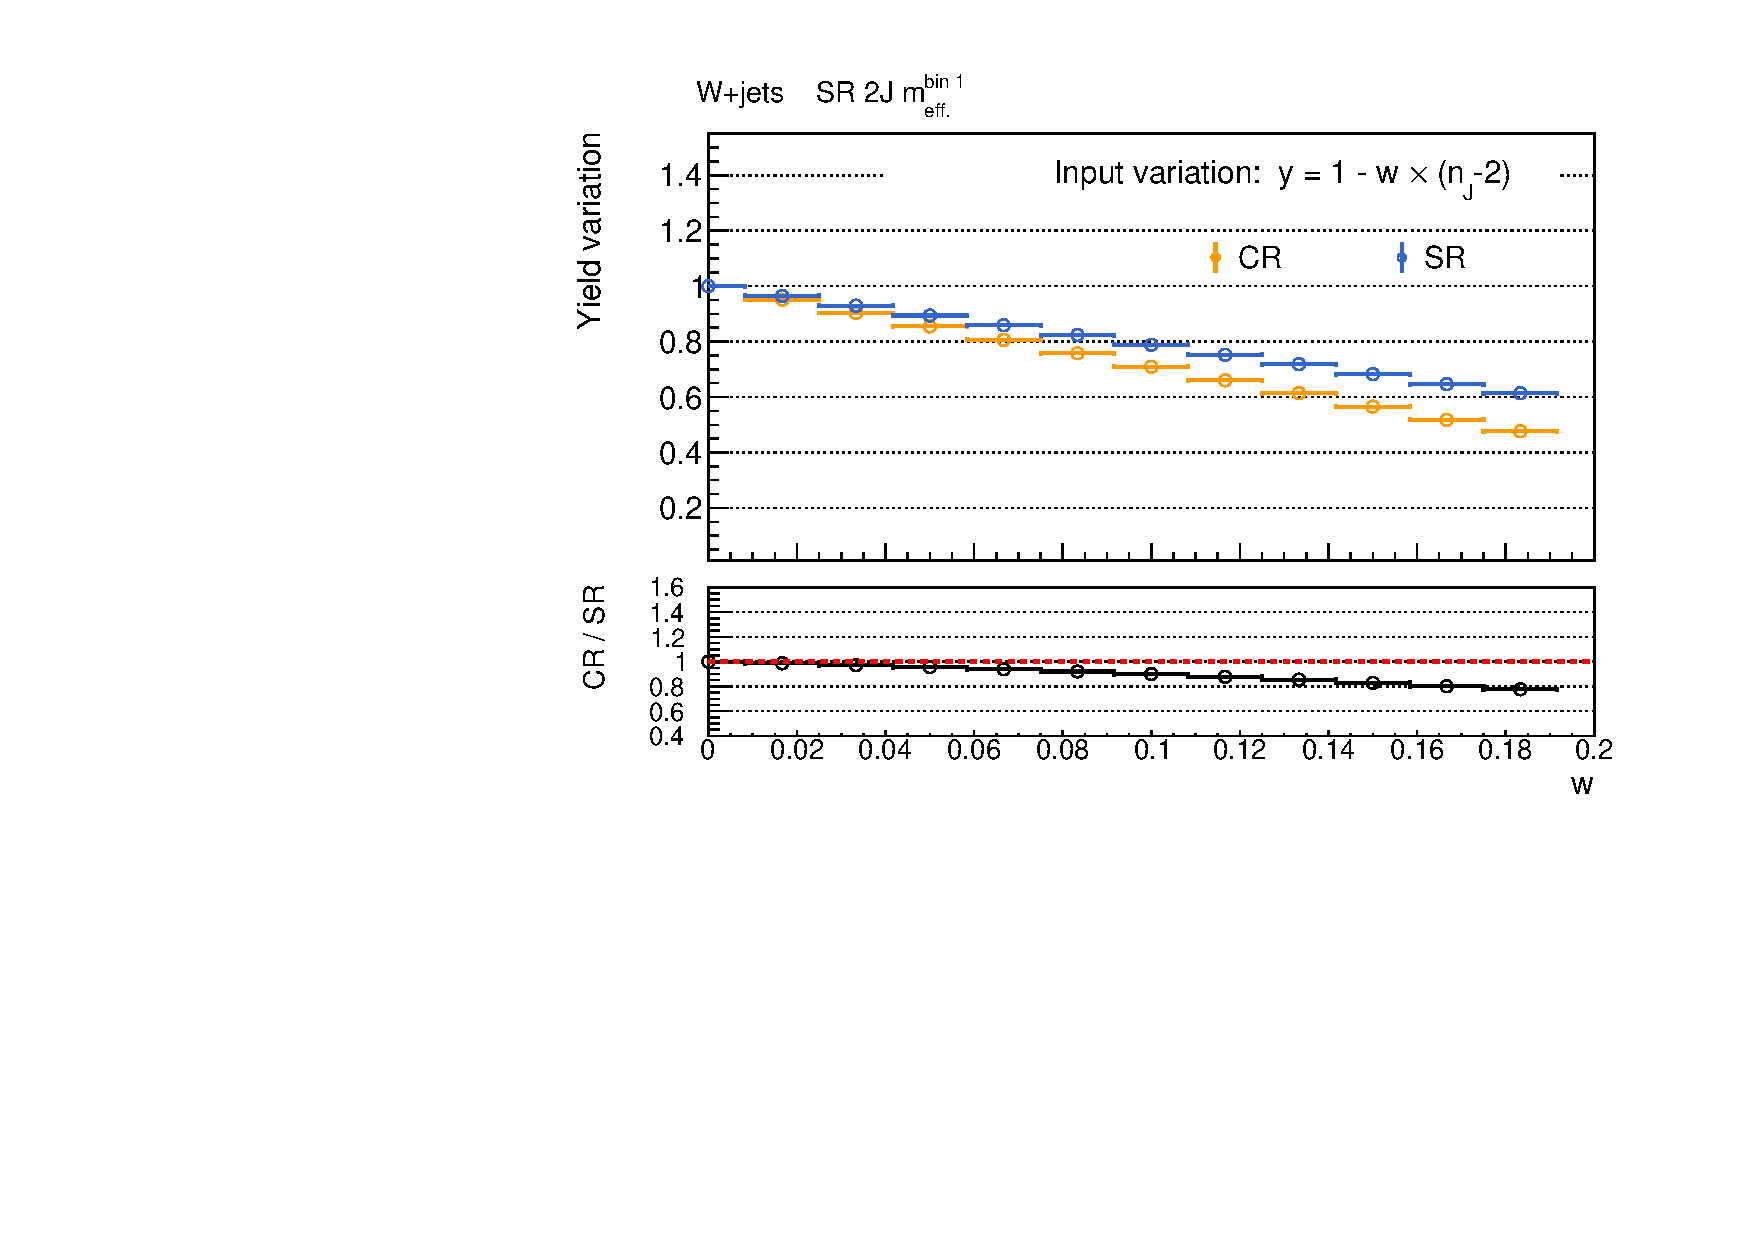
\includegraphics[width=0.488\textwidth]{figures/BGestimation/valid_extp/SFTF_wjets_SR2JMEFF1_extp_var2J__nJet30.pdf}}
    \subfigure[]{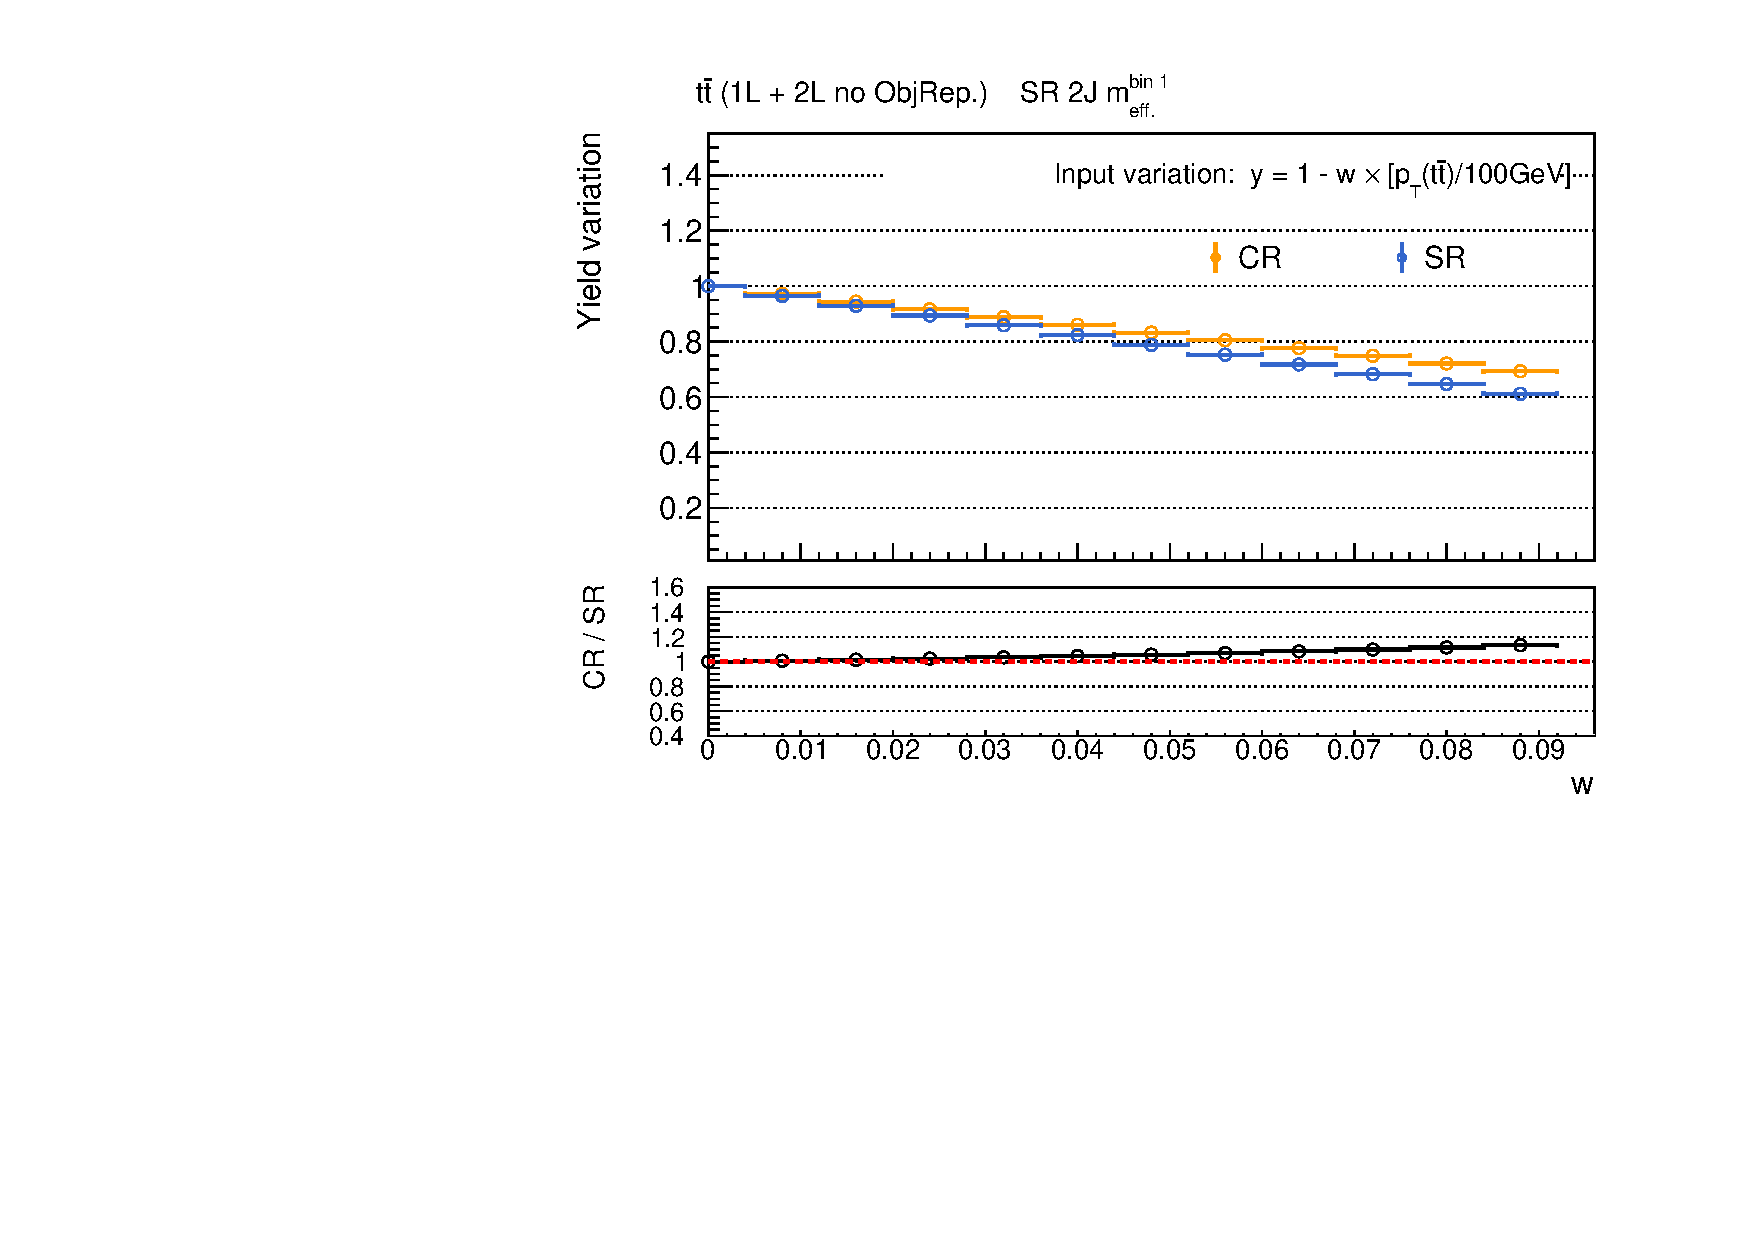
\includegraphics[width=0.488\textwidth]{figures/BGestimation/valid_extp/SFTF_ttNoObjRep_SR2JMEFF1_extp_var2J__ttPt.pdf}}
    \subfigure[]{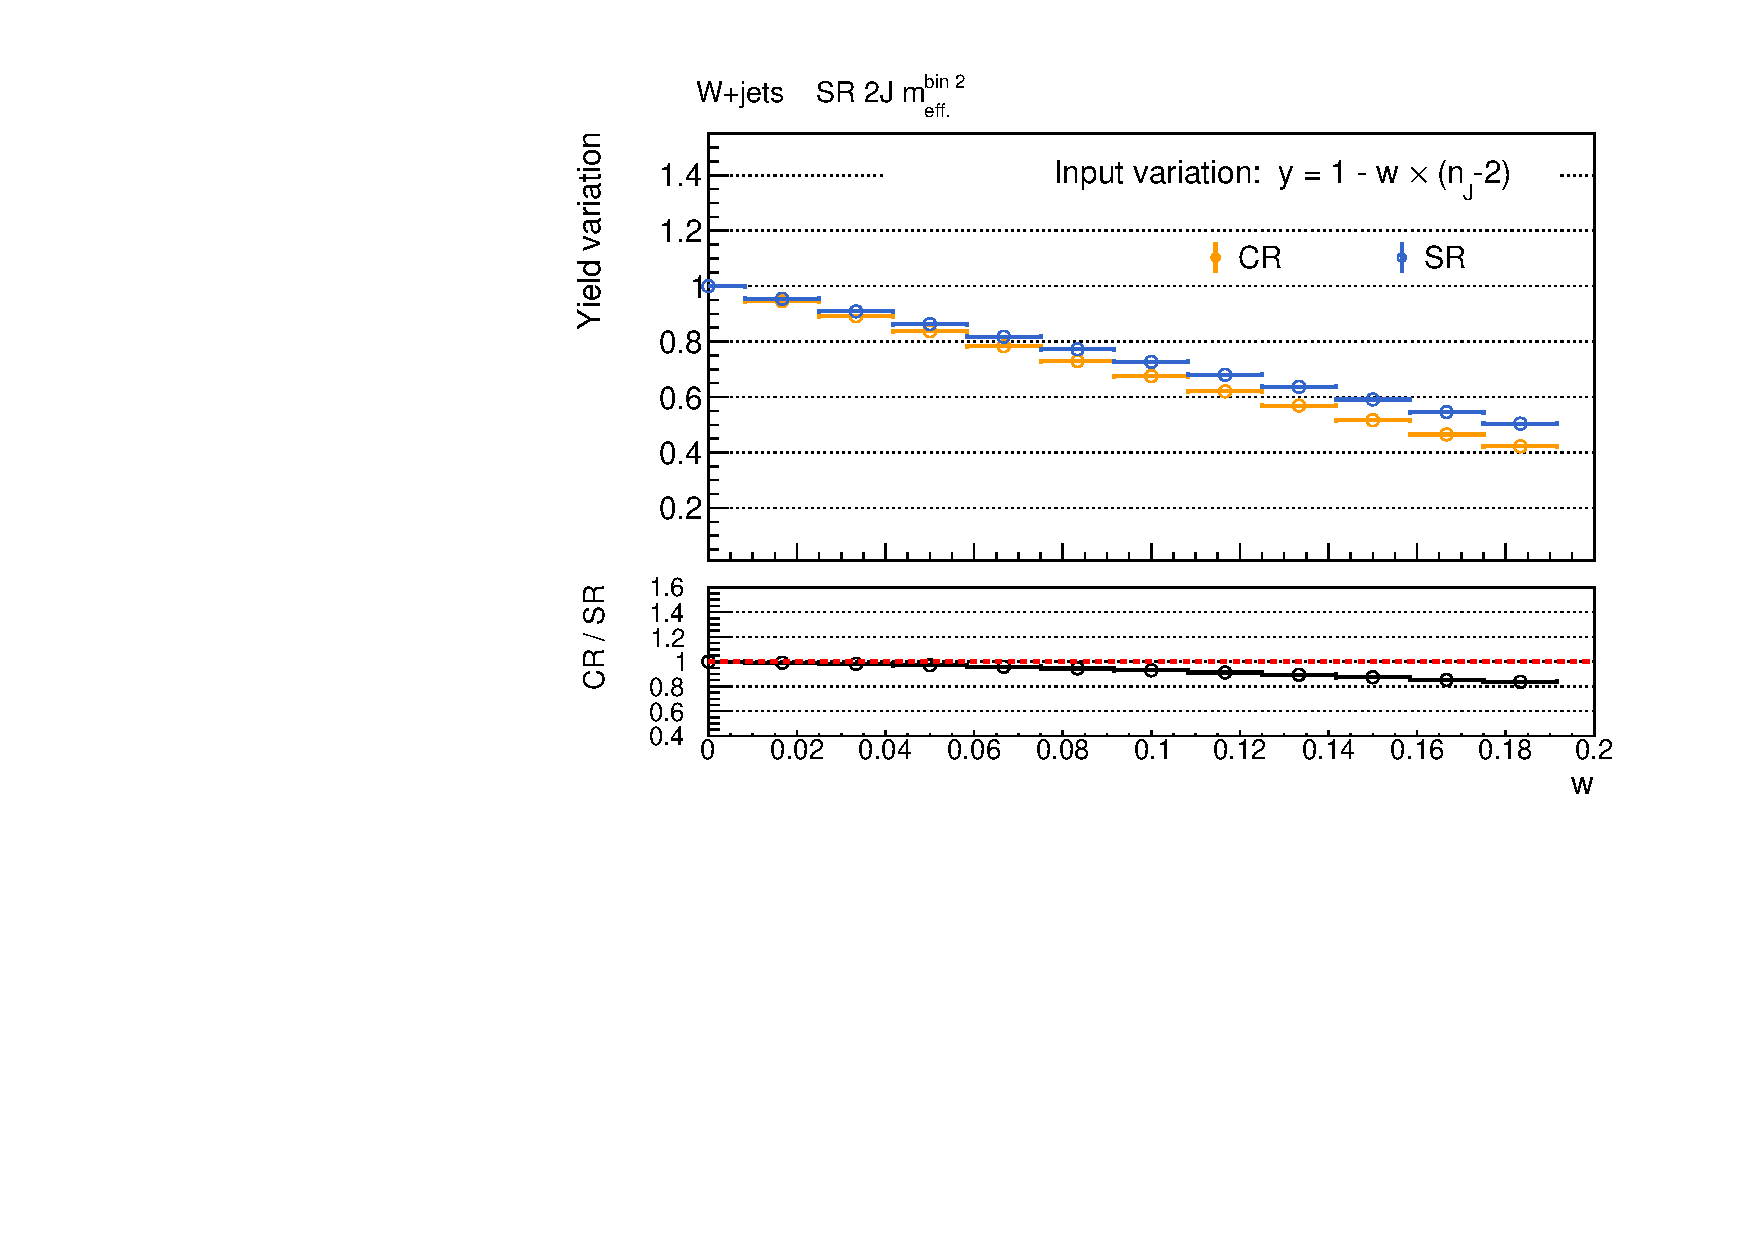
\includegraphics[width=0.488\textwidth]{figures/BGestimation/valid_extp/SFTF_wjets_SR2JMEFF2_extp_var2J__nJet30.pdf}}
    \subfigure[]{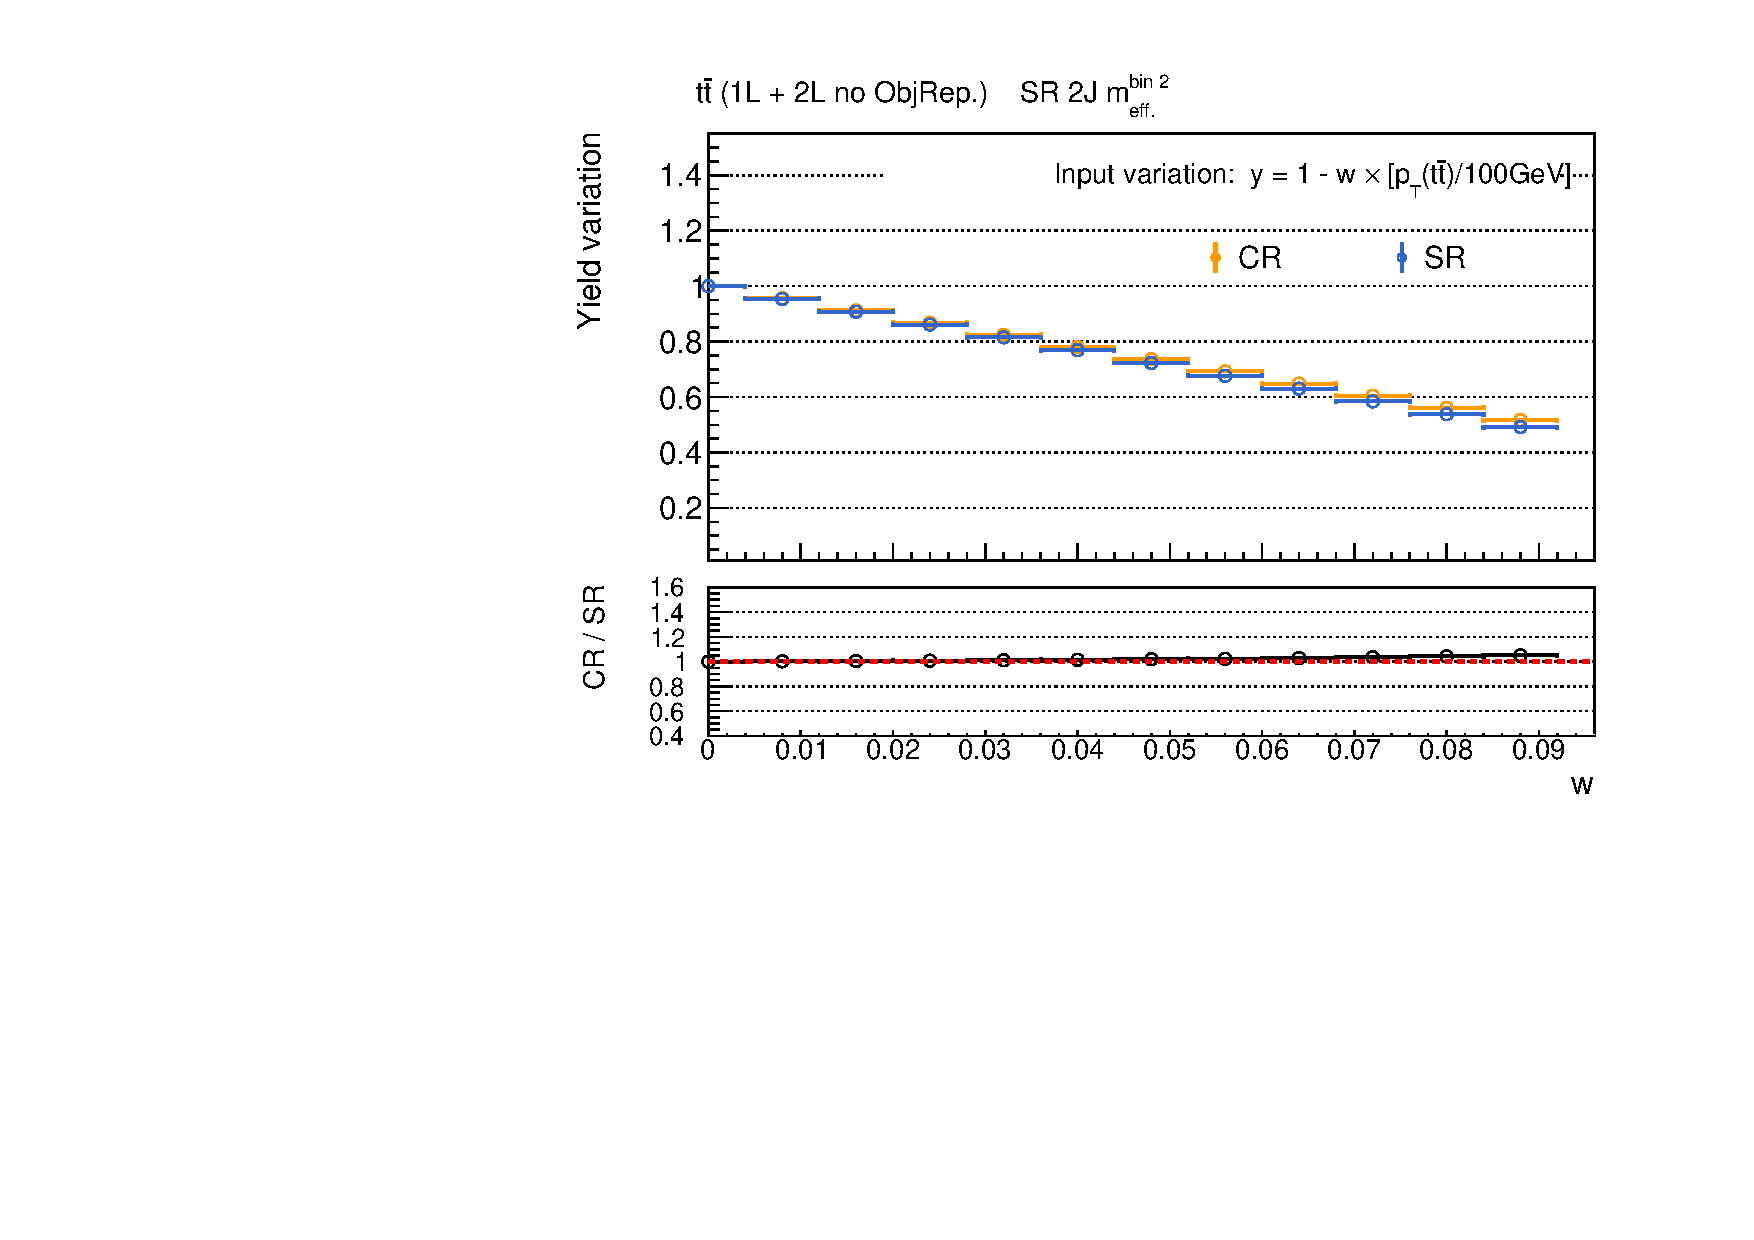
\includegraphics[width=0.488\textwidth]{figures/BGestimation/valid_extp/SFTF_ttNoObjRep_SR2JMEFF2_extp_var2J__ttPt.pdf}}
    \subfigure[]{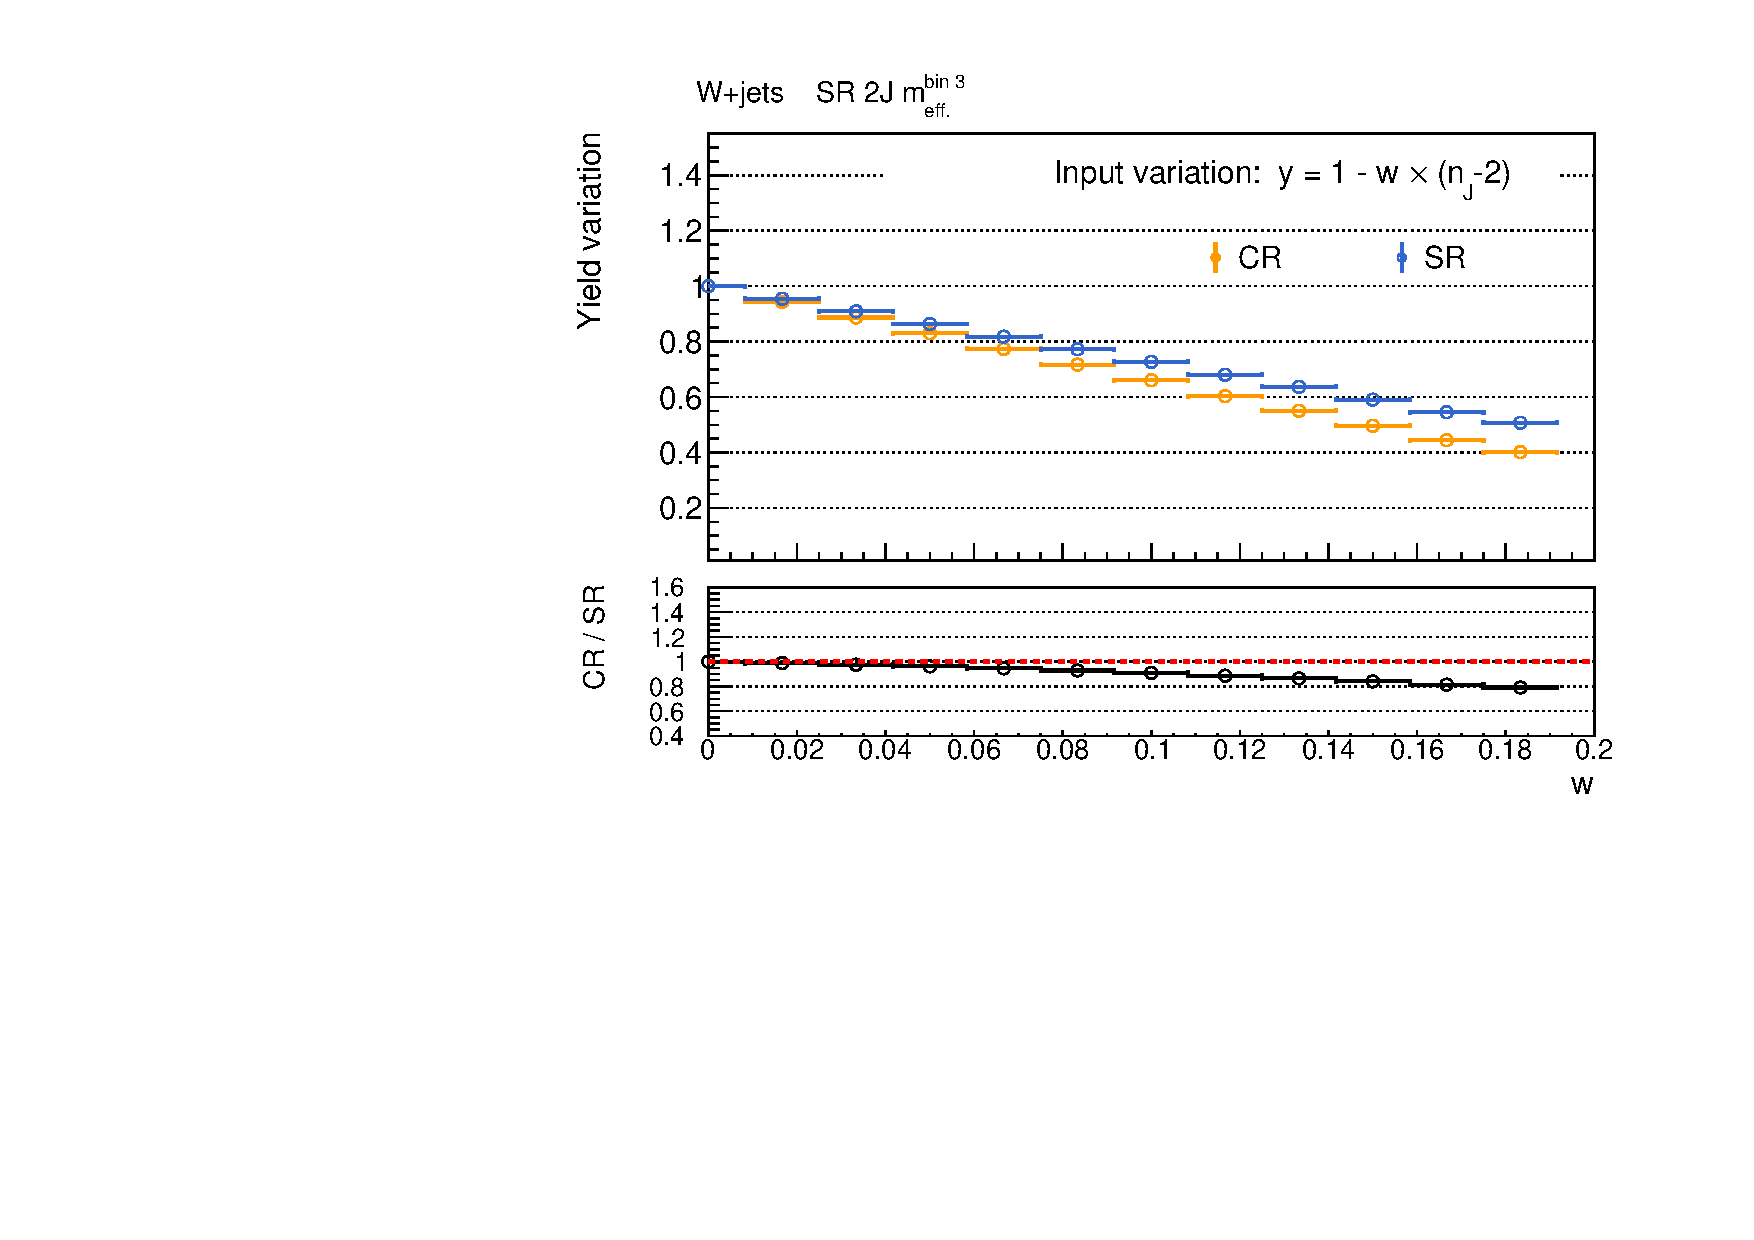
\includegraphics[width=0.488\textwidth]{figures/BGestimation/valid_extp/SFTF_wjets_SR2JMEFF3_extp_var2J__nJet30.pdf}}
    \subfigure[]{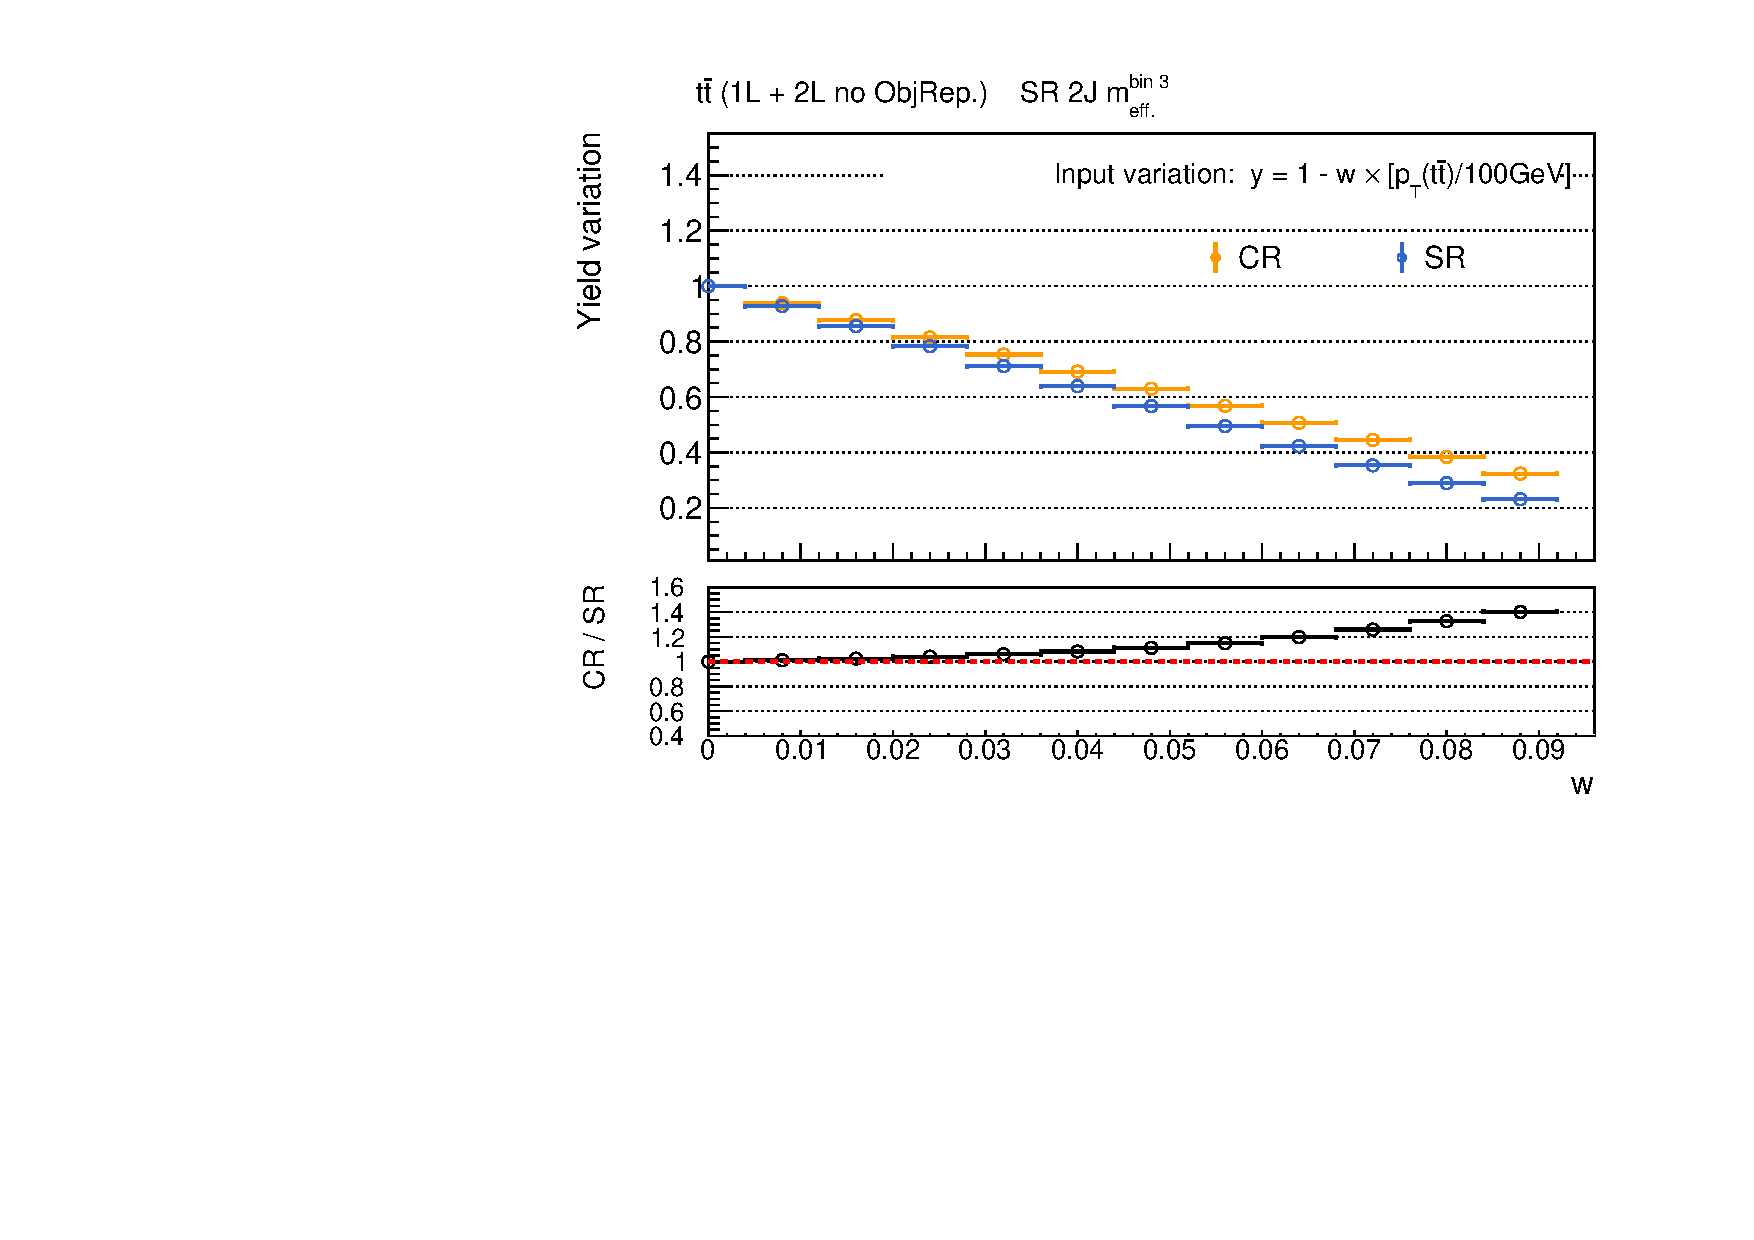
\includegraphics[width=0.488\textwidth]{figures/BGestimation/valid_extp/SFTF_ttNoObjRep_SR2JMEFF3_extp_var2J__ttPt.pdf}}
 \caption{Extrapolation error in SR/CR 2J. B-tagging requirement is removed. Top pannels show the yield variation of (a) $\wjets$ and (b) $\ttbar$ when injecting the variation by reweighting the MC with Eq. \ref{eq::BGestimation::injected_MCvariation}. Bottom rows are the relative difference in their response against the injected variation, namely the extrapolation errir. For the $\ttbar$ process, component estimated by the object replacement method is removed.  \label{fig::BGestimation::valid_extp_2J} }
\end{figure}



%%%%%%%%%%%%%%%% SR6J
\begin{figure}[h]
  \centering
    \subfigure[]{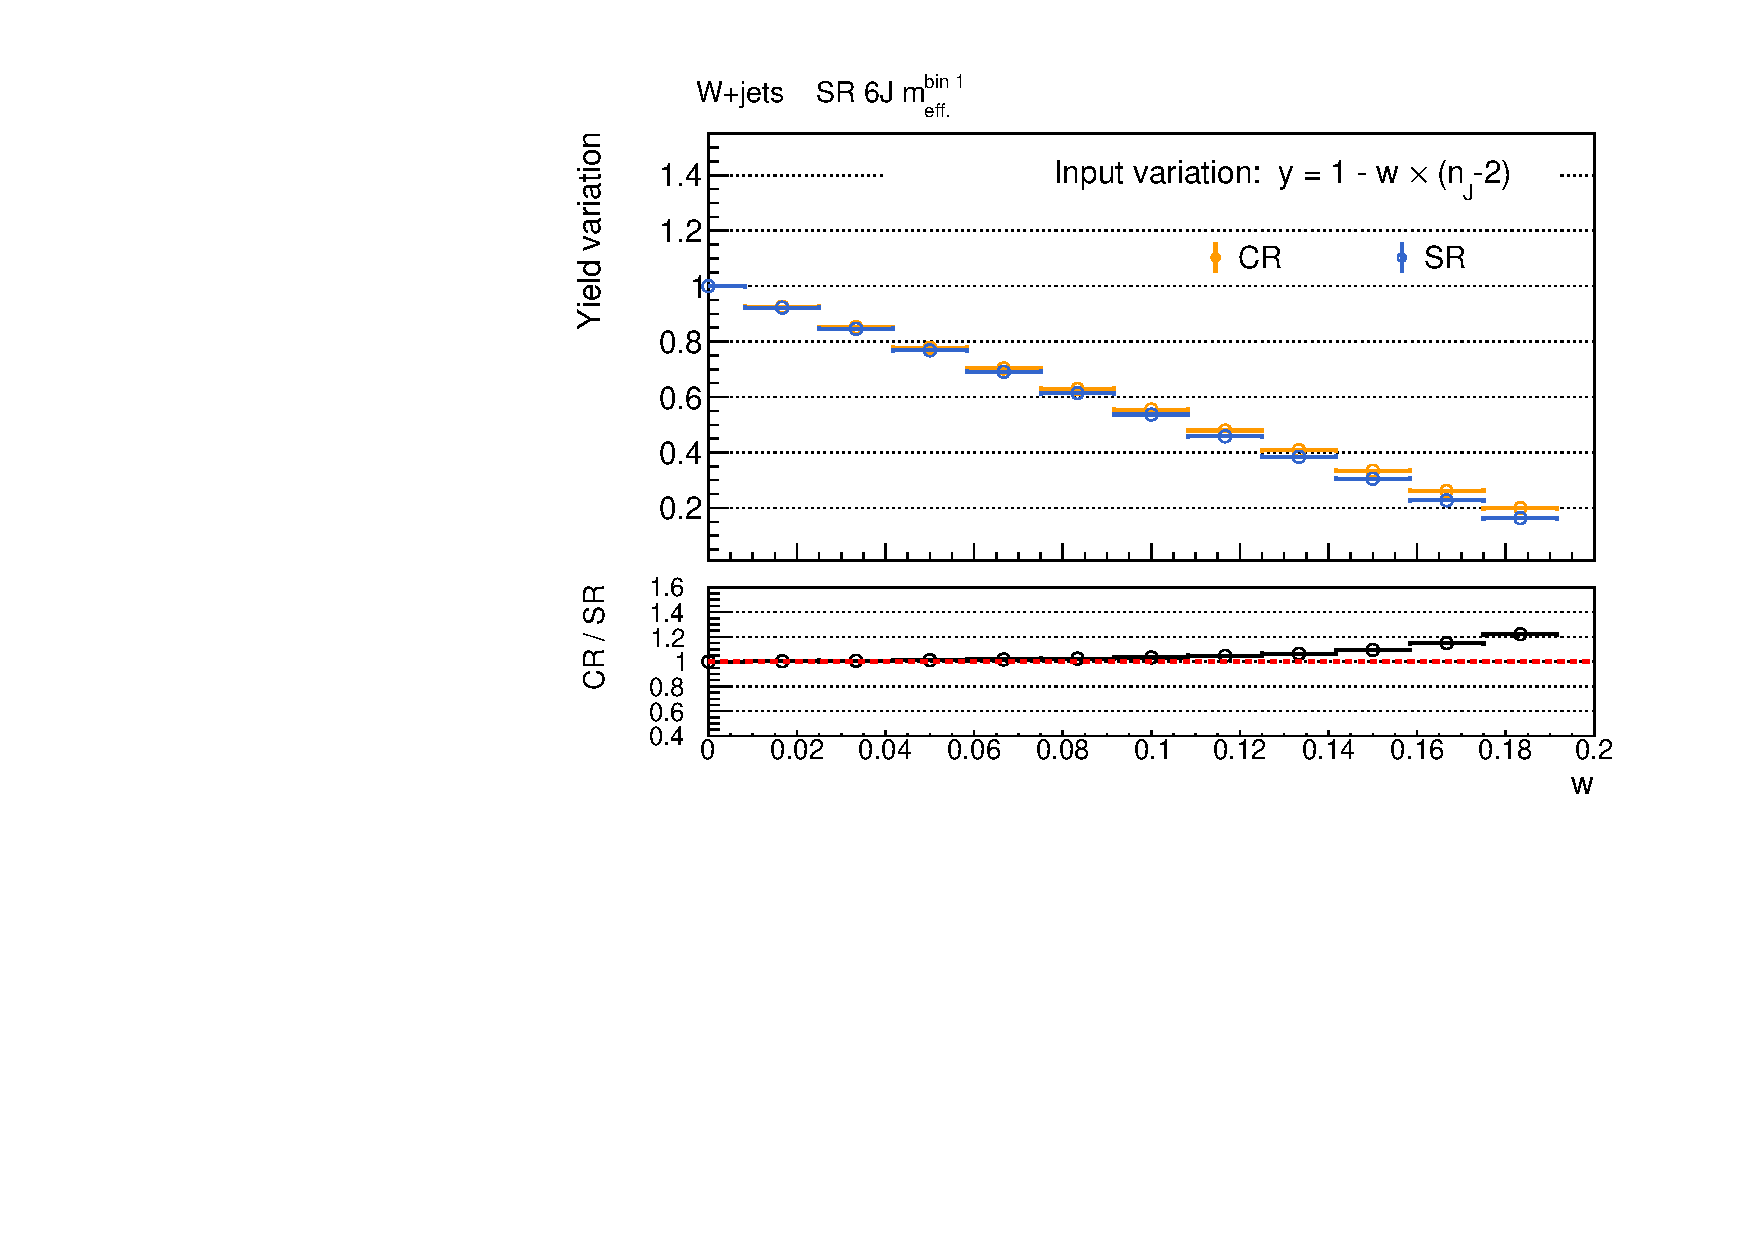
\includegraphics[width=0.488\textwidth]{figures/BGestimation/valid_extp/SFTF_wjets_SR6JMEFF1_extp_var6J__nJet30.pdf}}
    \subfigure[]{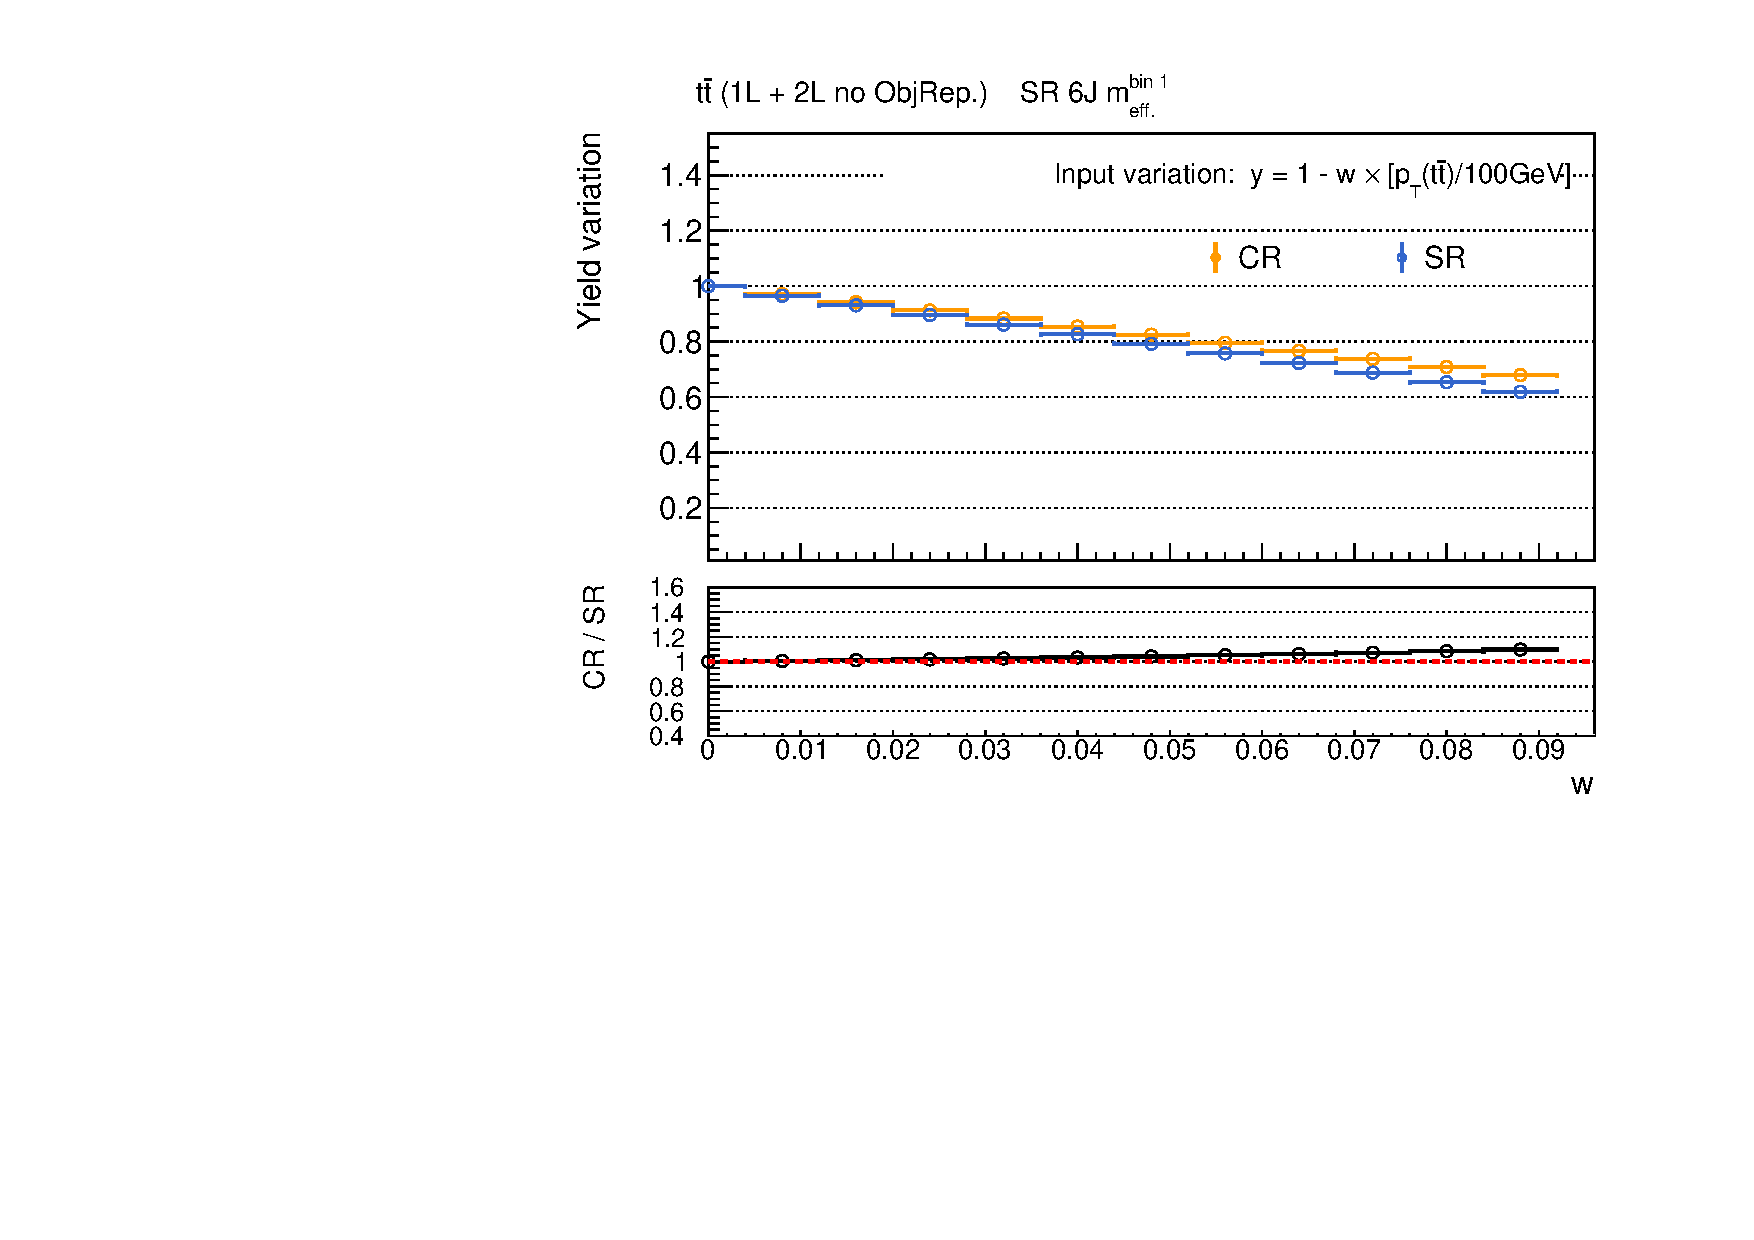
\includegraphics[width=0.488\textwidth]{figures/BGestimation/valid_extp/SFTF_ttNoObjRep_SR6JMEFF1_extp_var6J__ttPt.pdf}}
    \subfigure[]{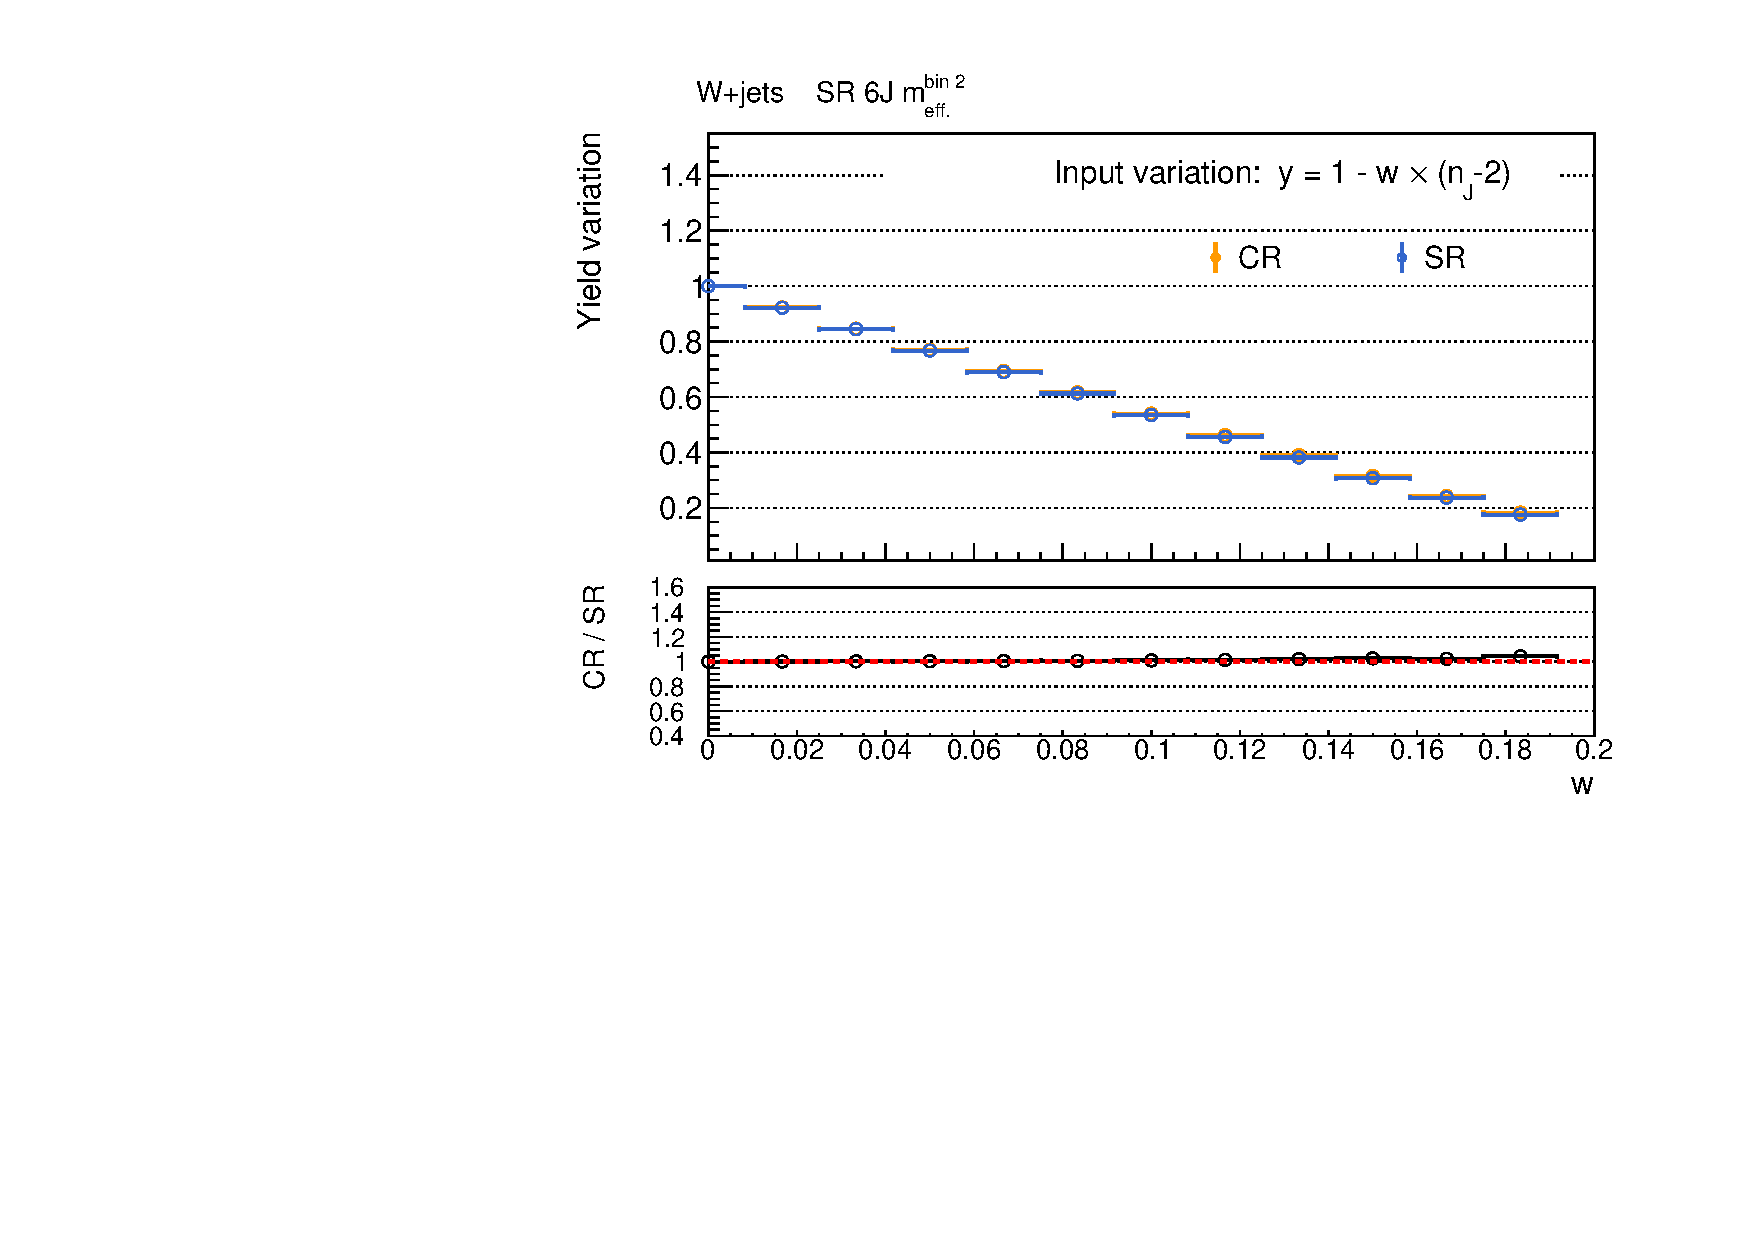
\includegraphics[width=0.488\textwidth]{figures/BGestimation/valid_extp/SFTF_wjets_SR6JMEFF2_extp_var6J__nJet30.pdf}}
    \subfigure[]{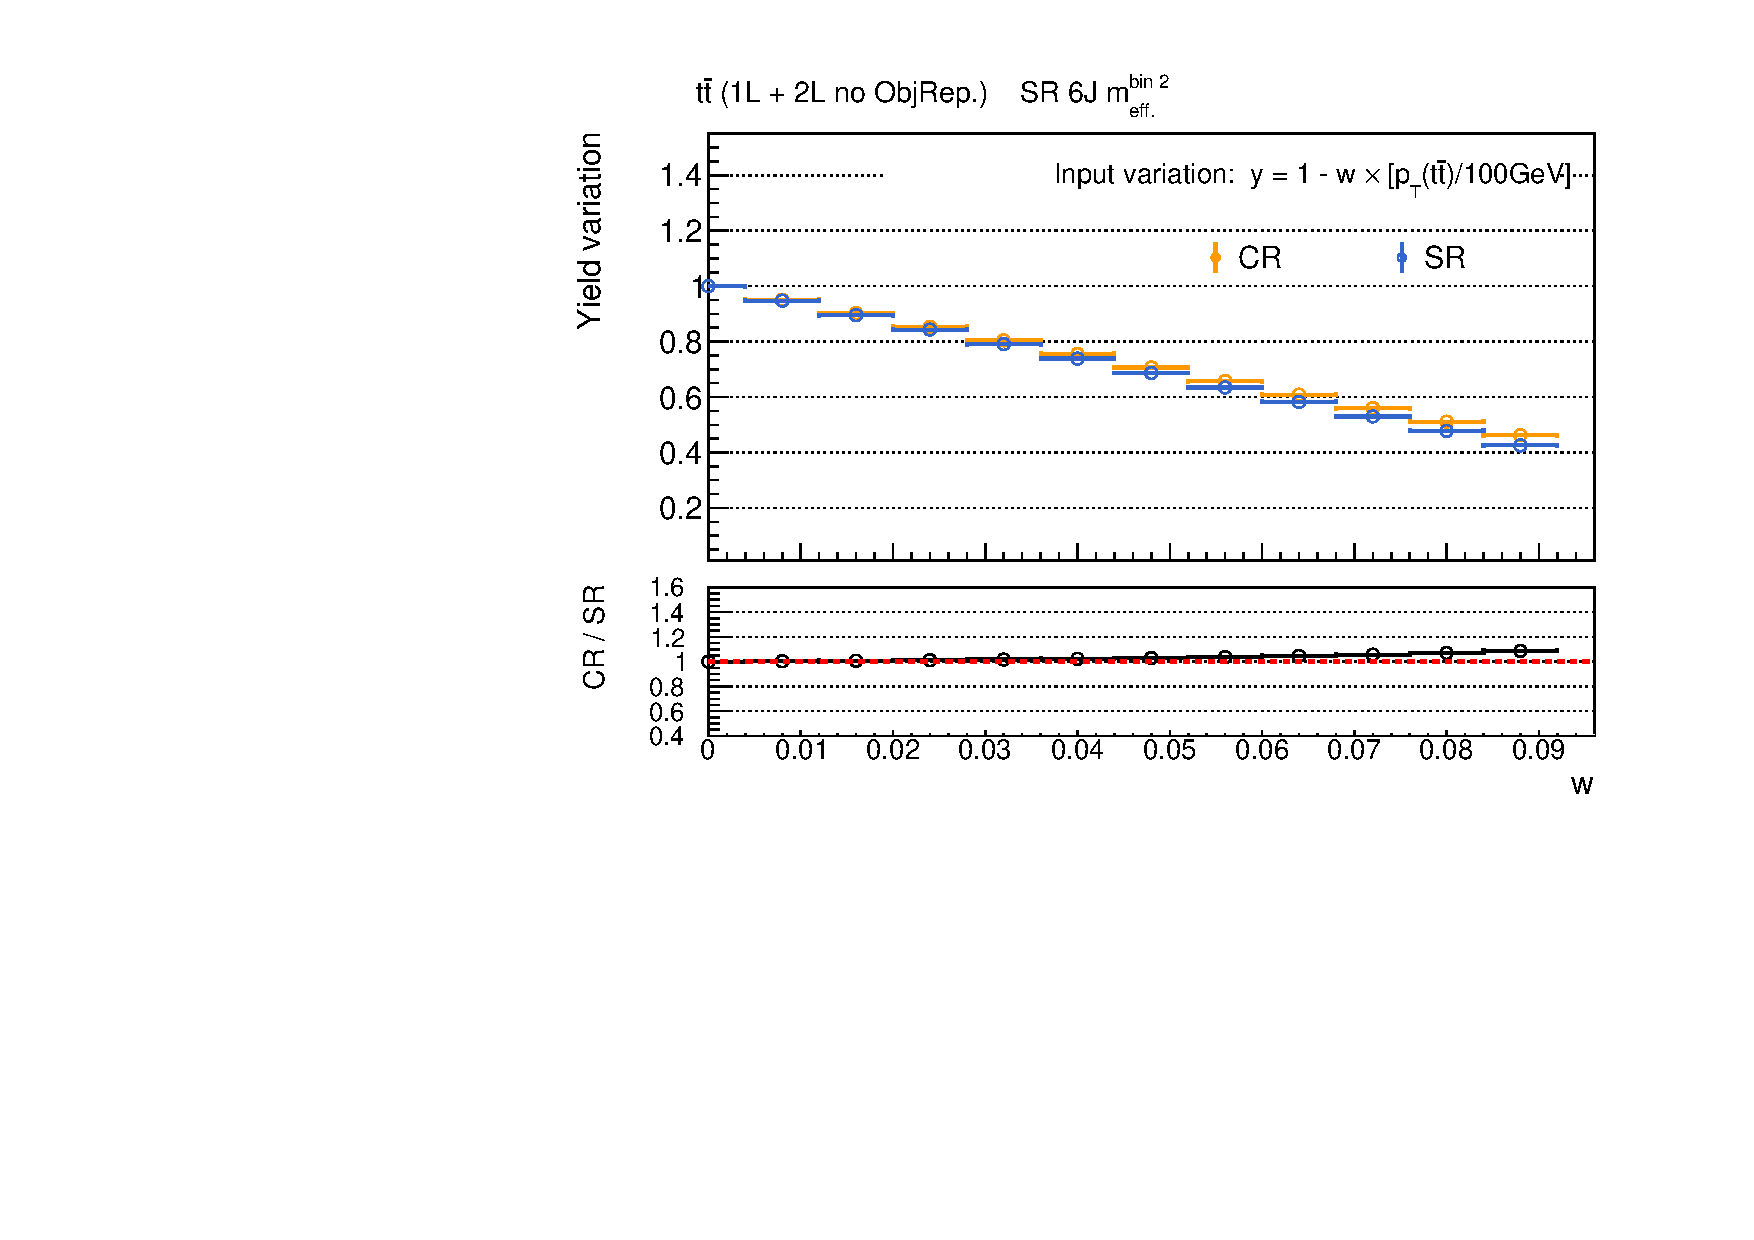
\includegraphics[width=0.488\textwidth]{figures/BGestimation/valid_extp/SFTF_ttNoObjRep_SR6JMEFF2_extp_var6J__ttPt.pdf}}
    \subfigure[]{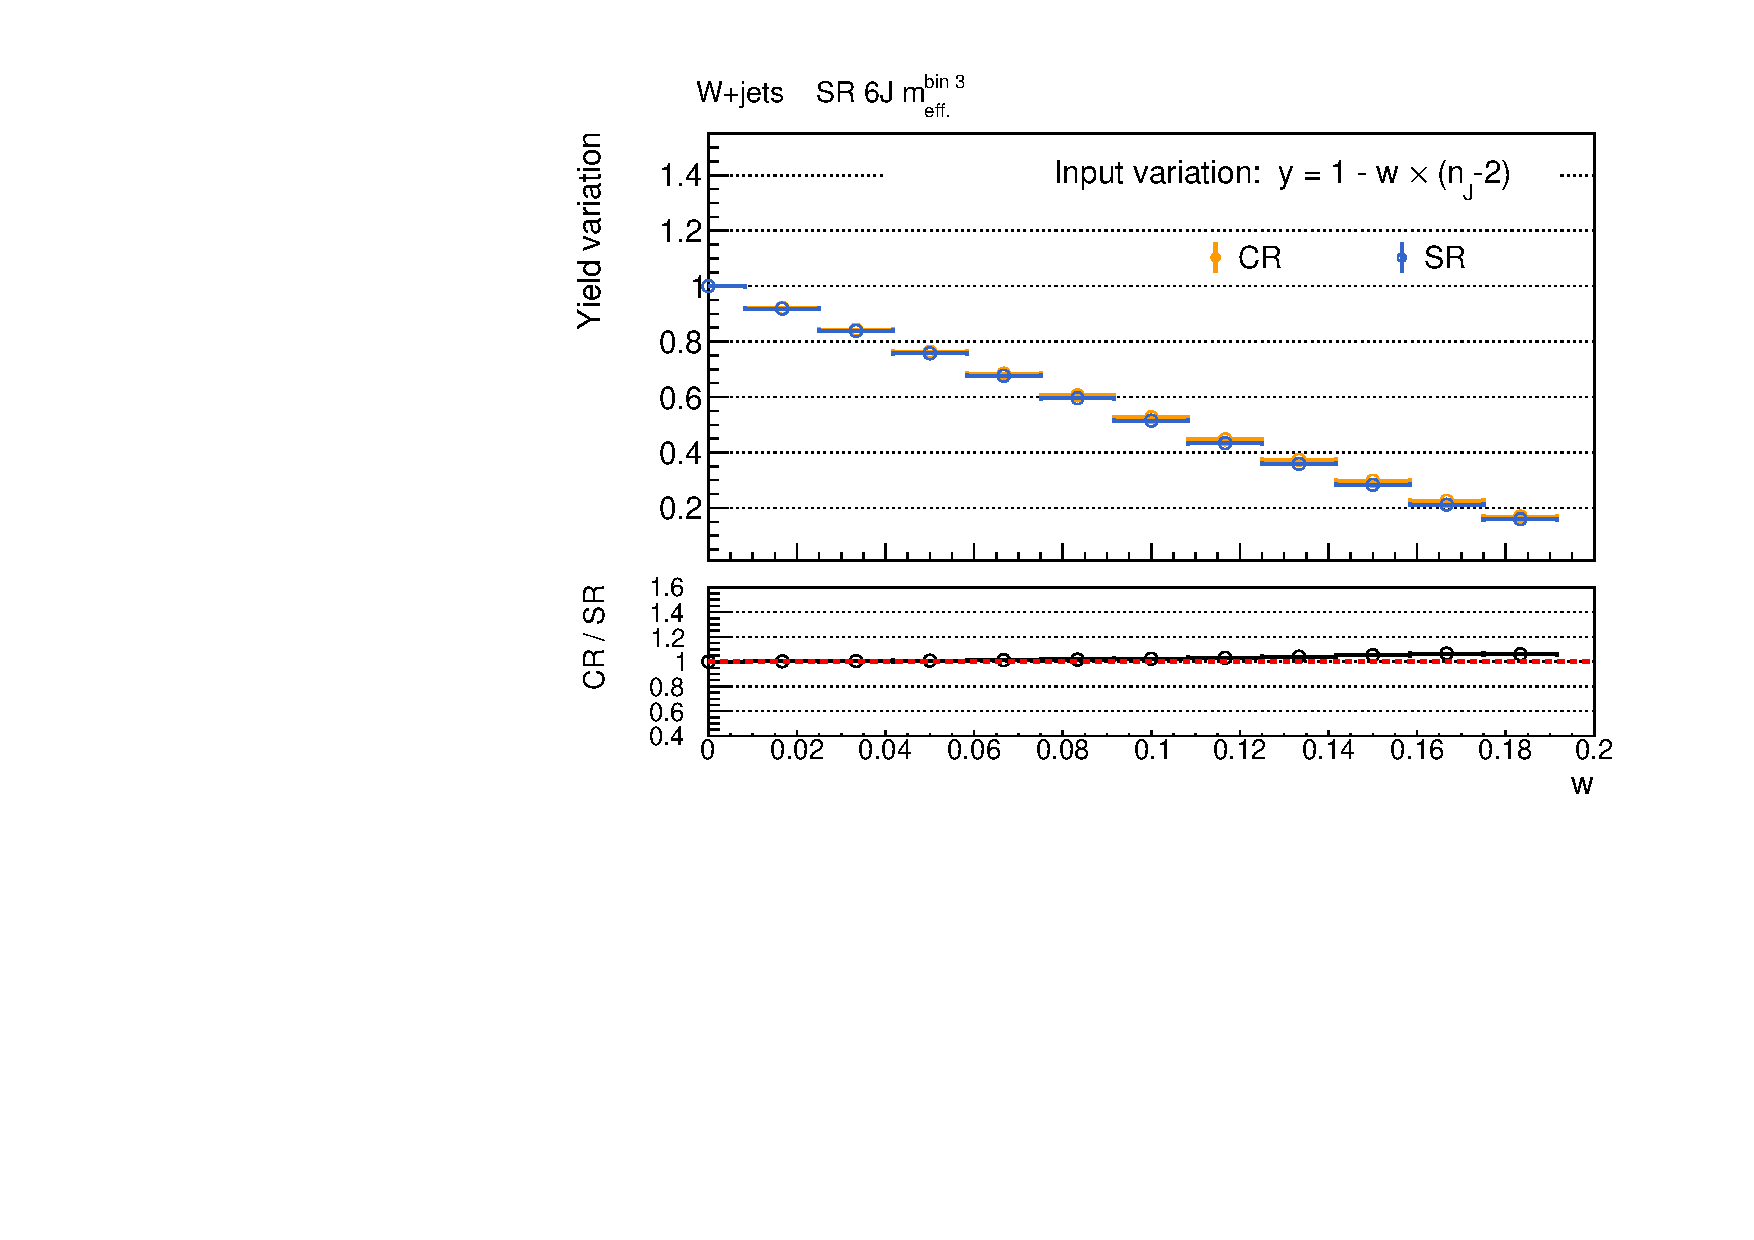
\includegraphics[width=0.488\textwidth]{figures/BGestimation/valid_extp/SFTF_wjets_SR6JMEFF3_extp_var6J__nJet30.pdf}}
    \subfigure[]{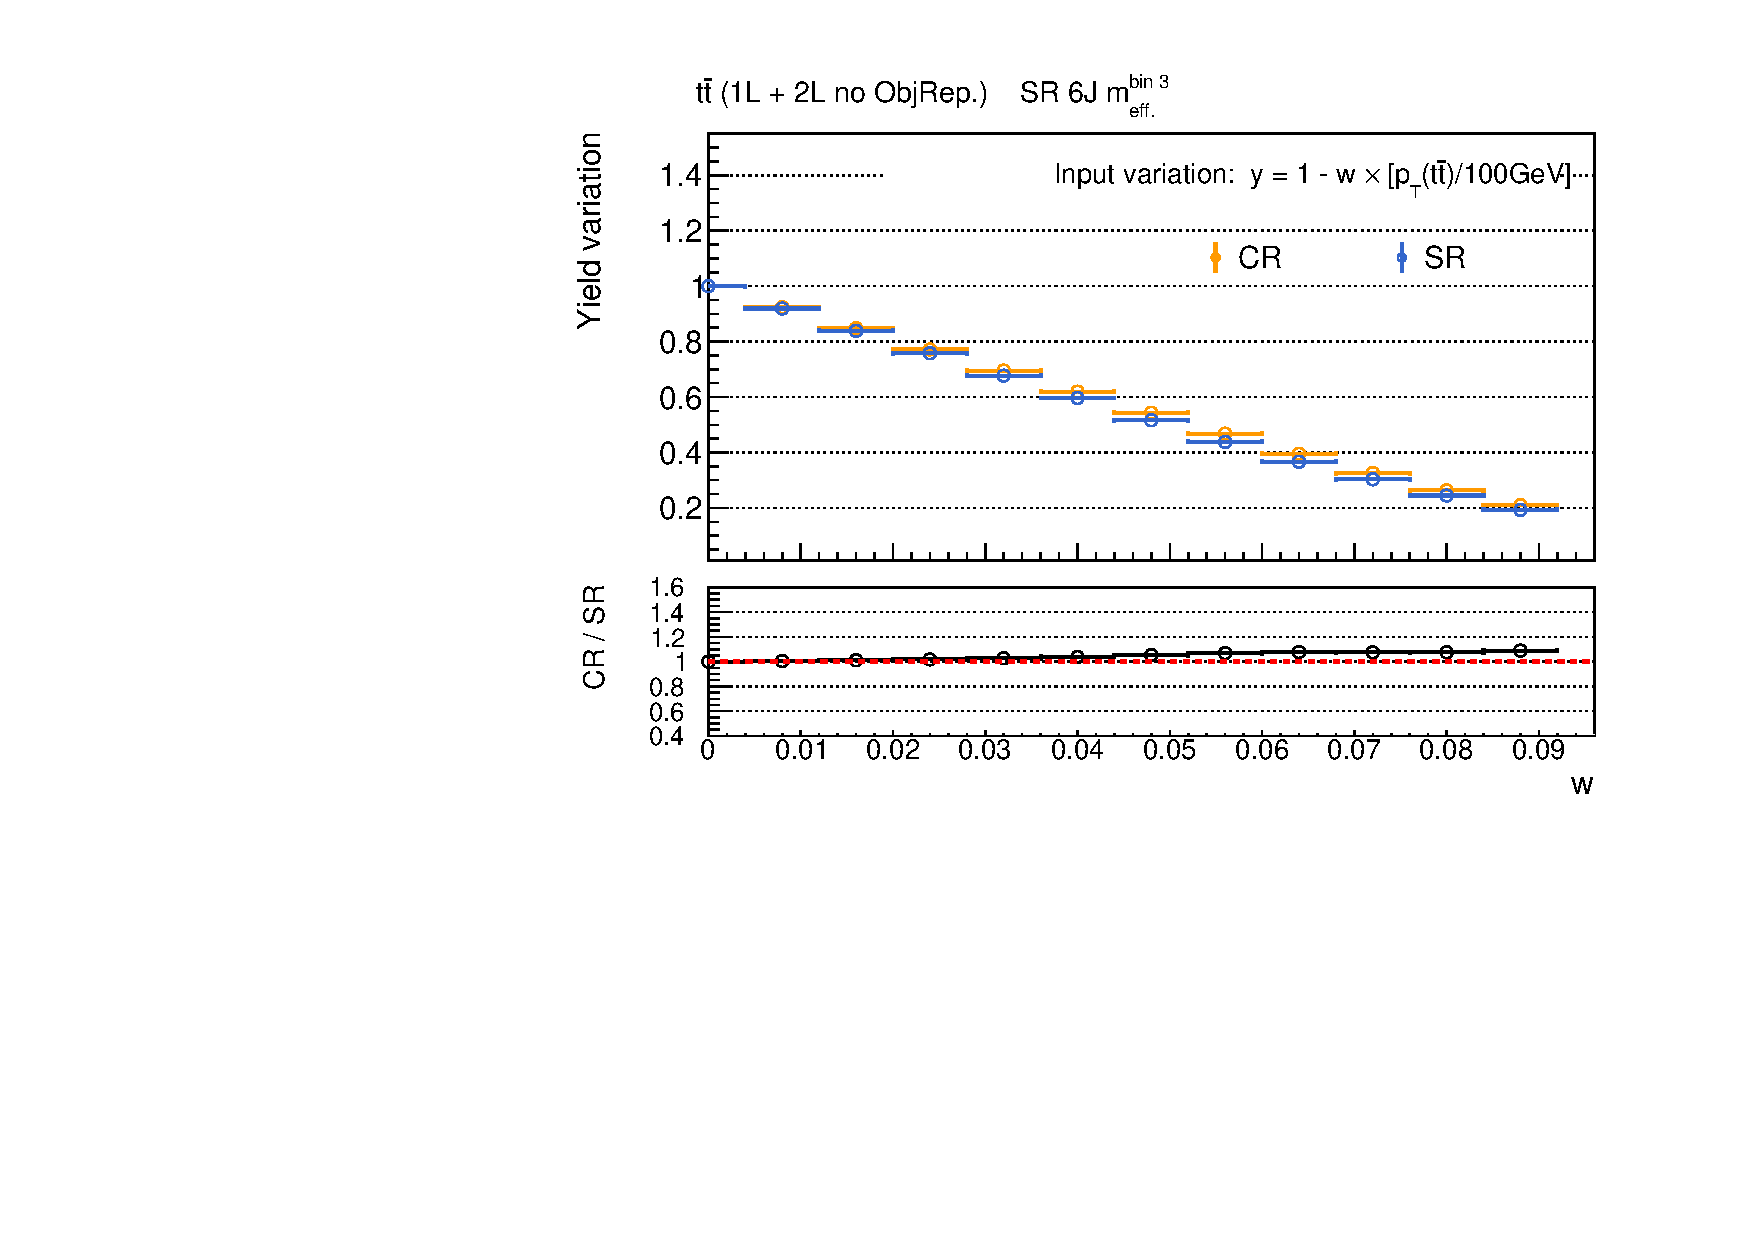
\includegraphics[width=0.488\textwidth]{figures/BGestimation/valid_extp/SFTF_ttNoObjRep_SR6JMEFF3_extp_var6J__ttPt.pdf}}
 \caption{Extrapolation error in SR/CR 6J. B-tagging requirement is removed. Top pannels show the yield variation of (a) $\wjets$ and (b) $\ttbar$ when injecting the variation by reweighting the MC with Eq. \ref{eq::BGestimation::injected_MCvariation}. Bottom rows are the relative difference in their response against the injected variation, namely the extrapolation errir. For the $\ttbar$ process, component estimated by the object replacement method is removed.  \label{fig::BGestimation::valid_extp_6J} }
\end{figure}


%%%%%%%%%%%%%%%% Lowx
\begin{figure}[h]
  \centering
    \subfigure[]{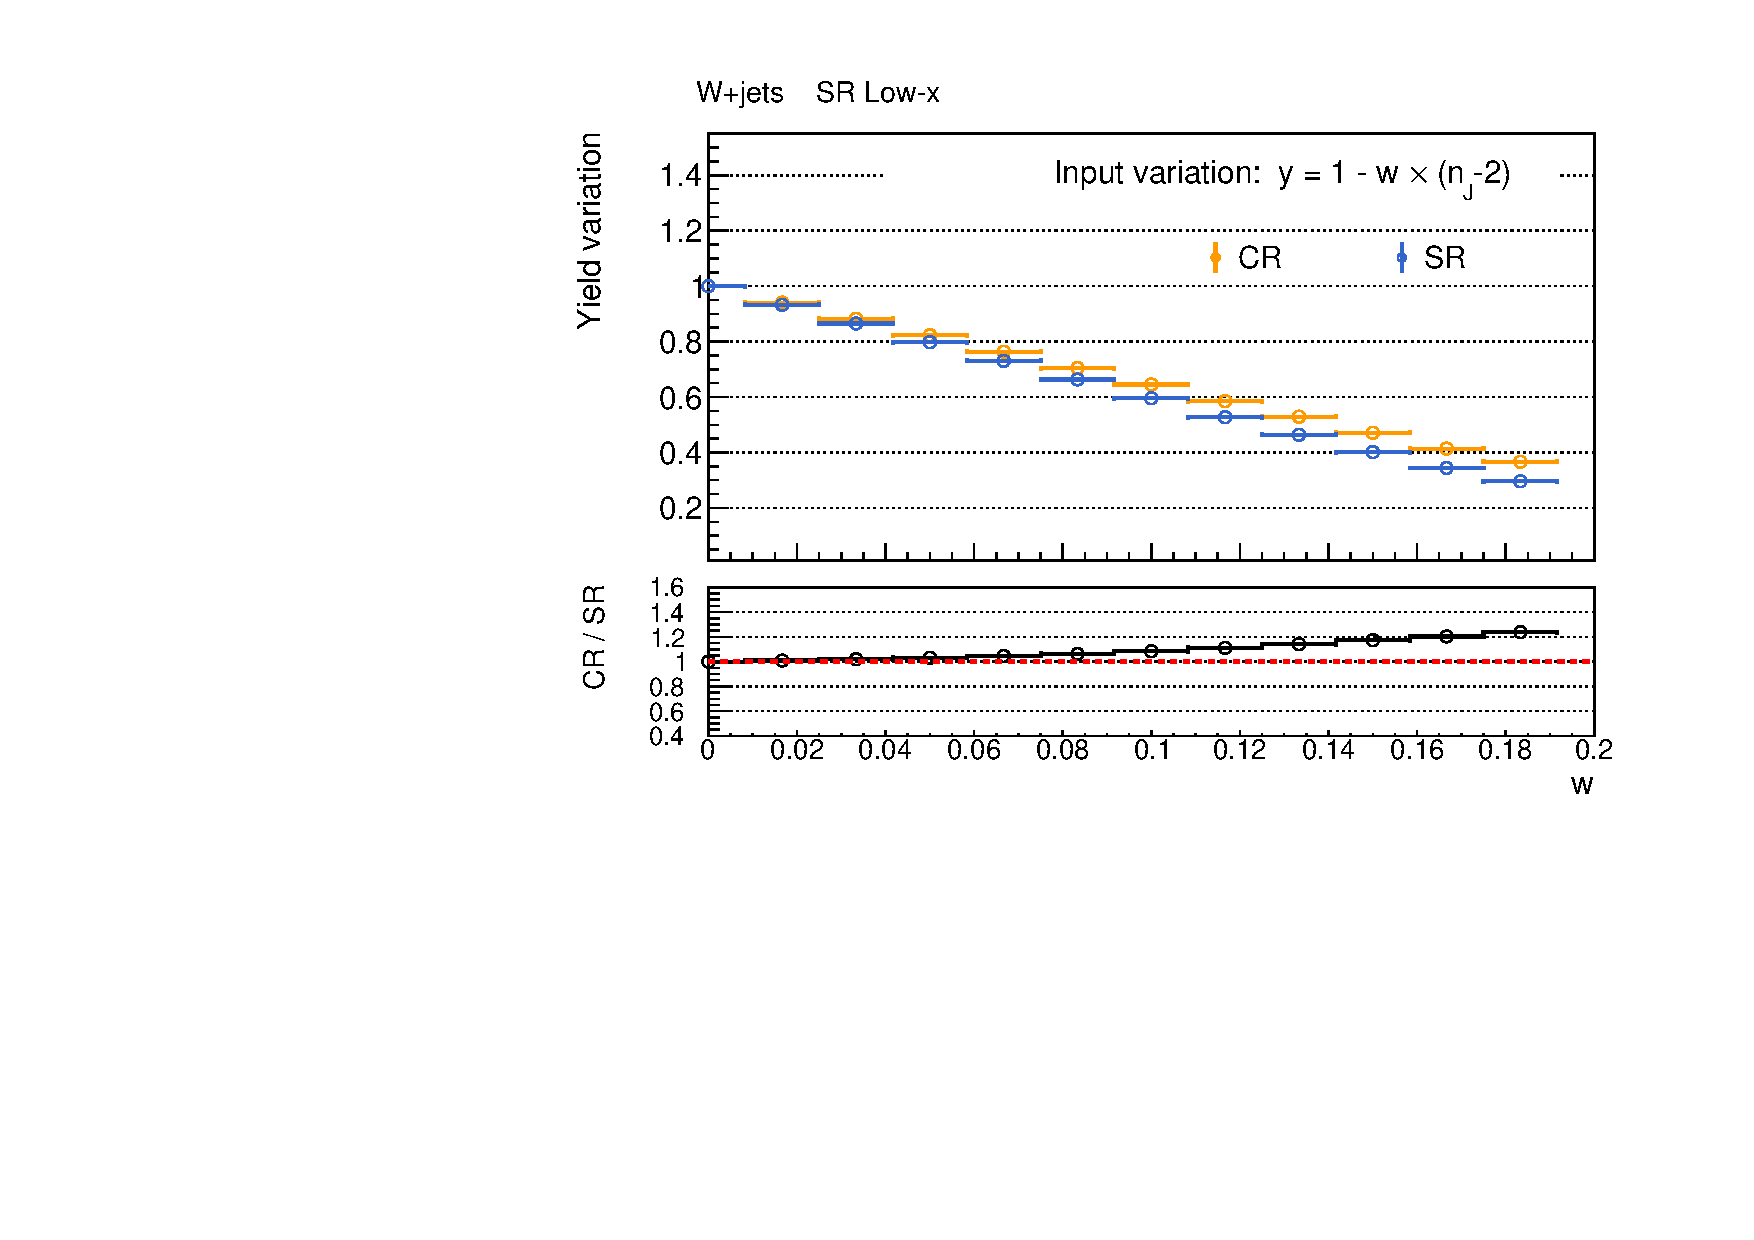
\includegraphics[width=0.488\textwidth]{figures/BGestimation/valid_extp/SFTF_wjets_SRLowx_extp_varLowx__nJet30.pdf}}
    \subfigure[]{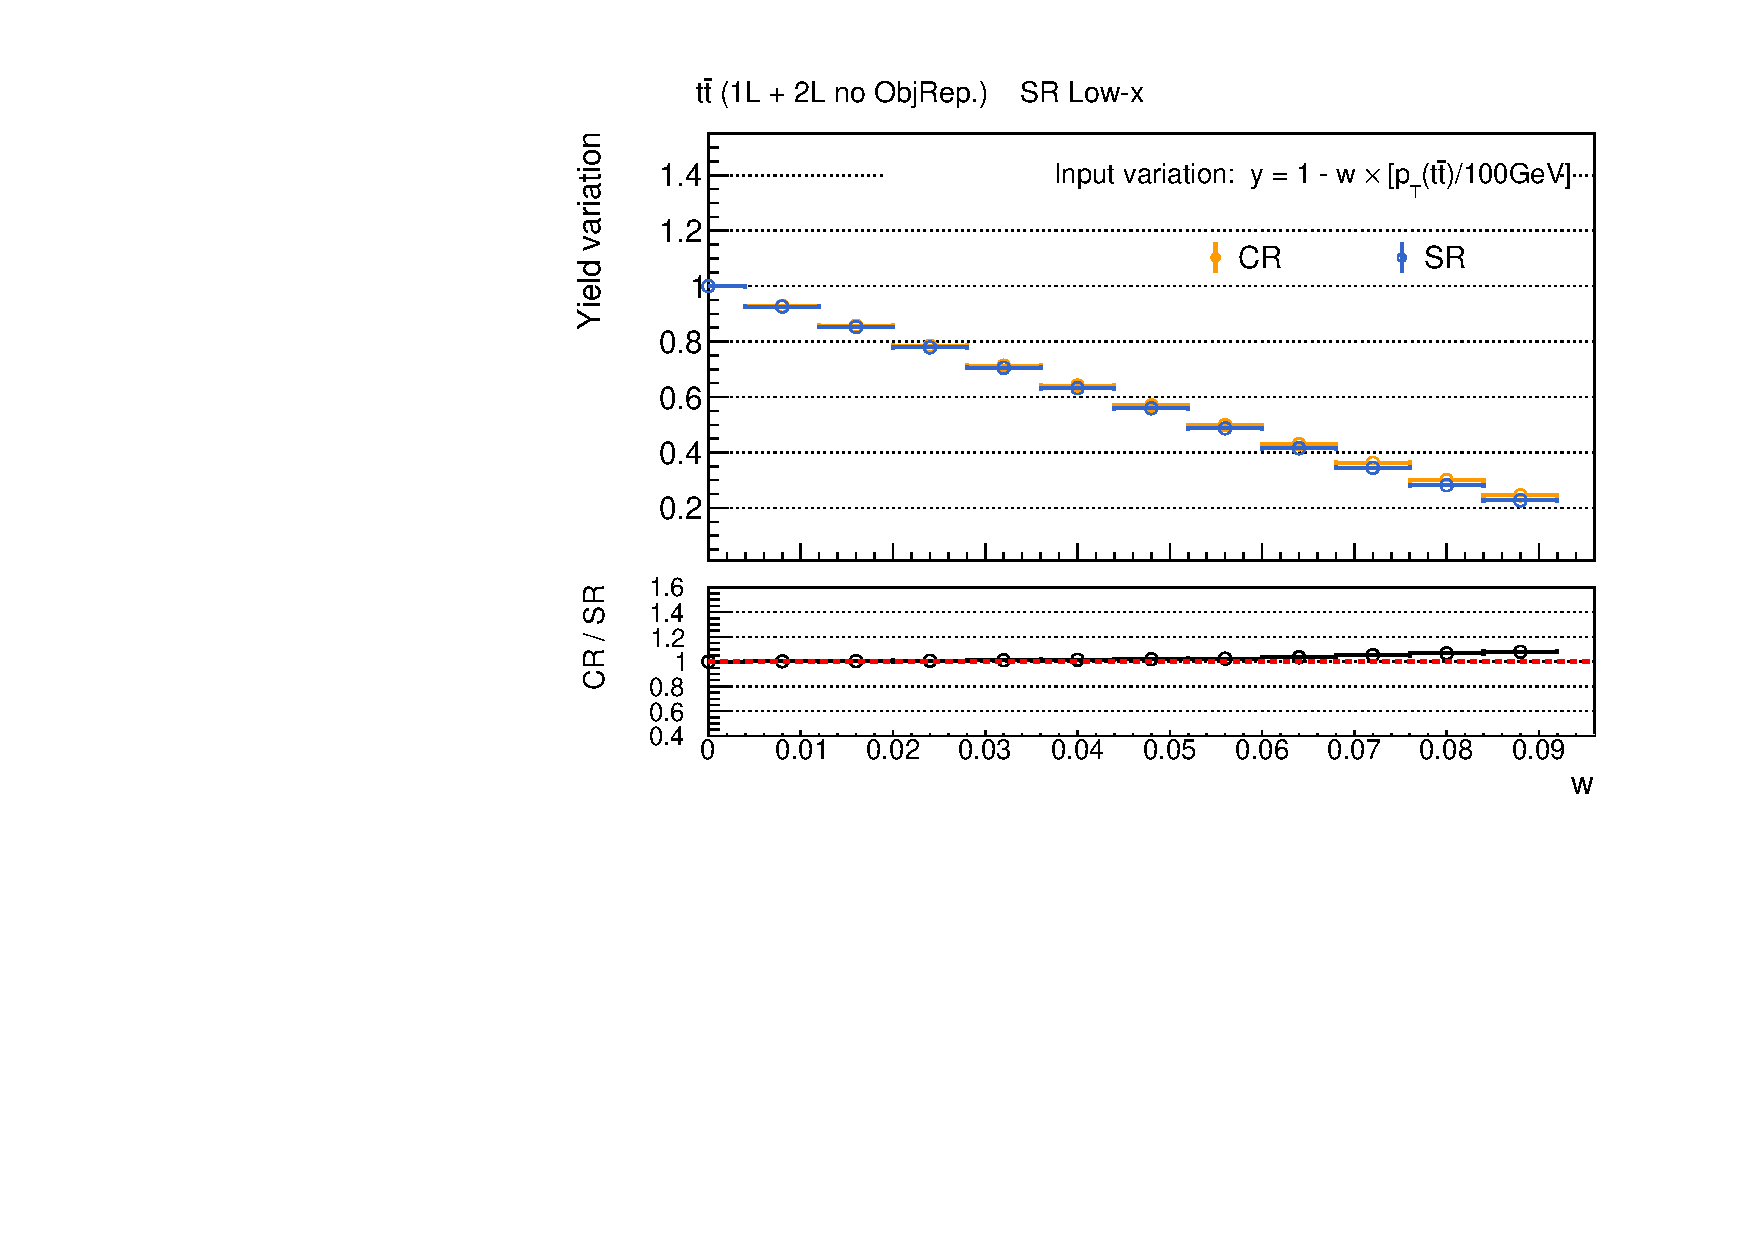
\includegraphics[width=0.488\textwidth]{figures/BGestimation/valid_extp/SFTF_ttNoObjRep_SRLowx_extp_varLowx__ttPt.pdf}}

%%%%%%%%%%%%%%%% Highx
    \subfigure[]{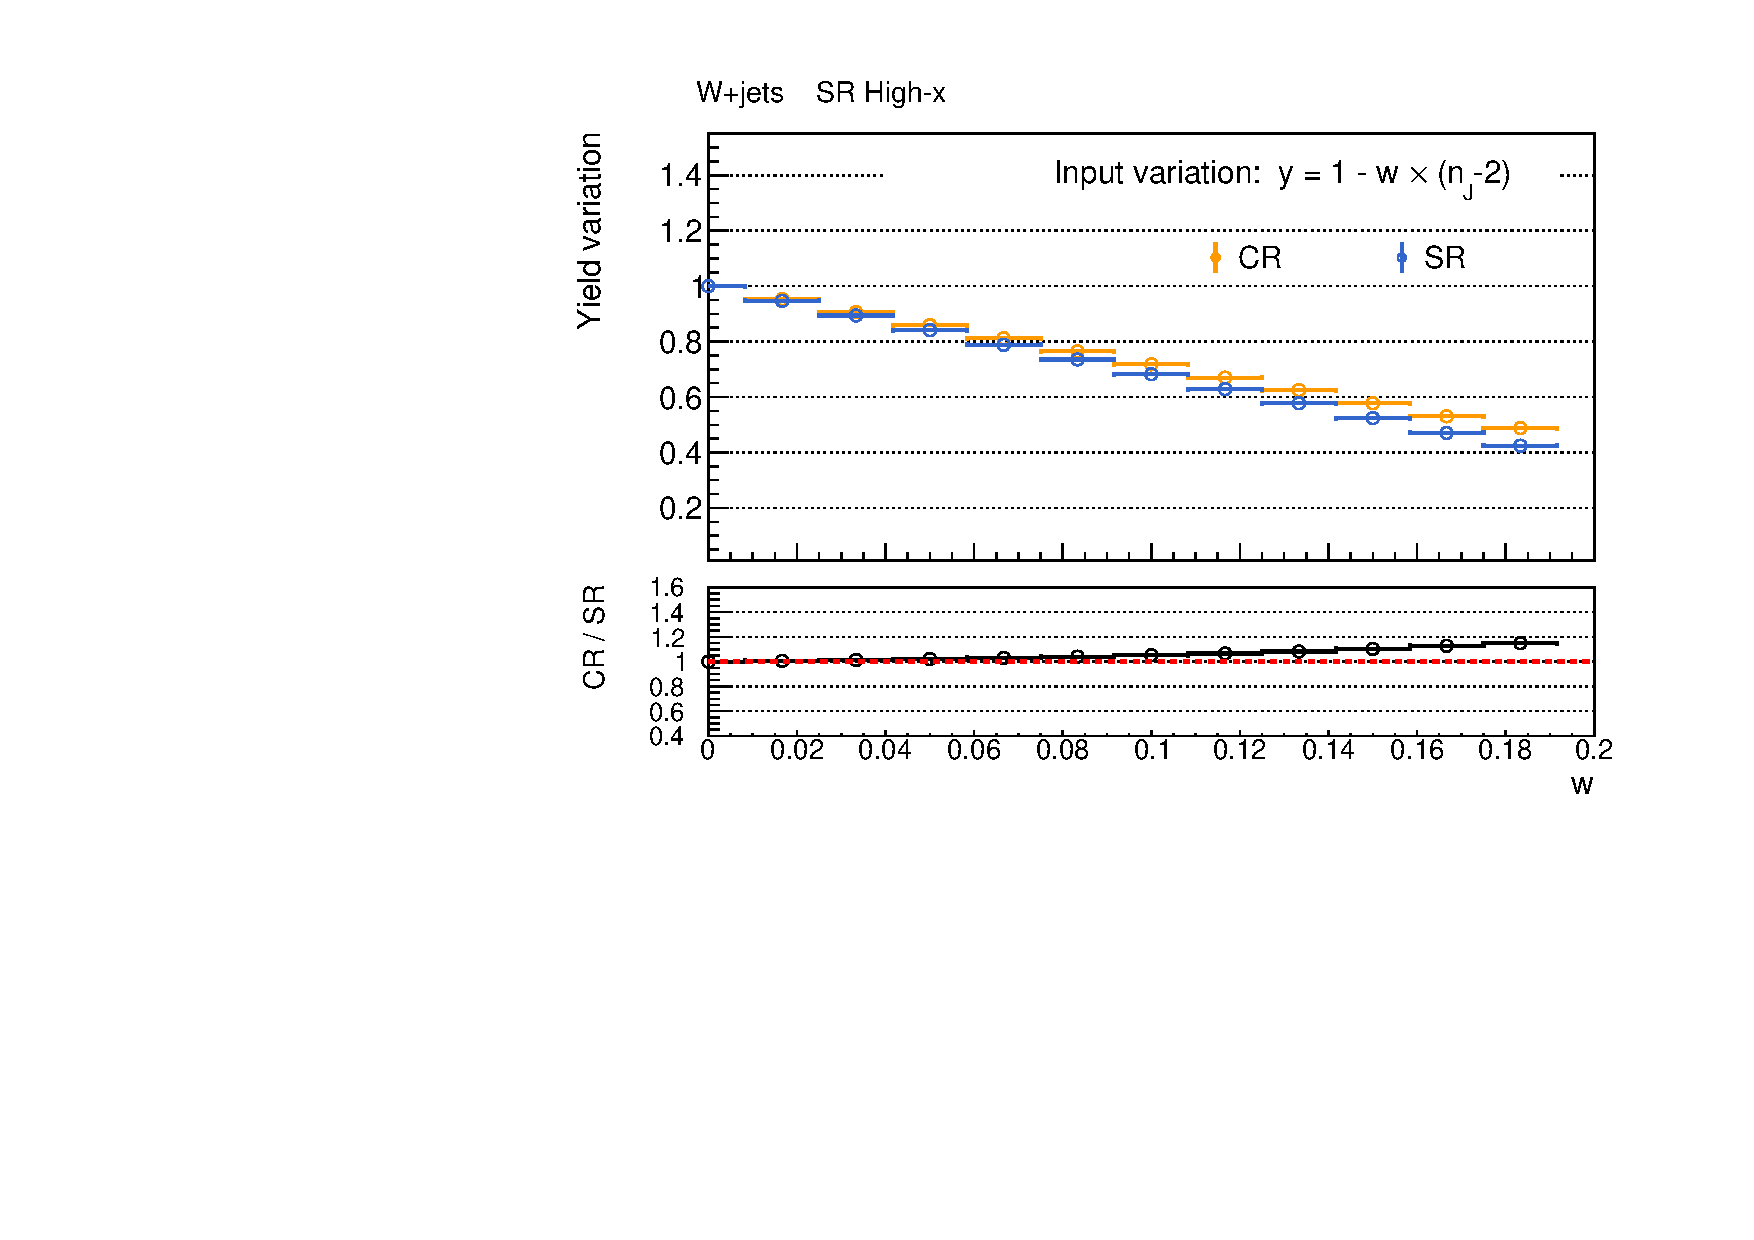
\includegraphics[width=0.488\textwidth]{figures/BGestimation/valid_extp/SFTF_wjets_SRHighx_extp_varHighx__nJet30.pdf}}
    \subfigure[]{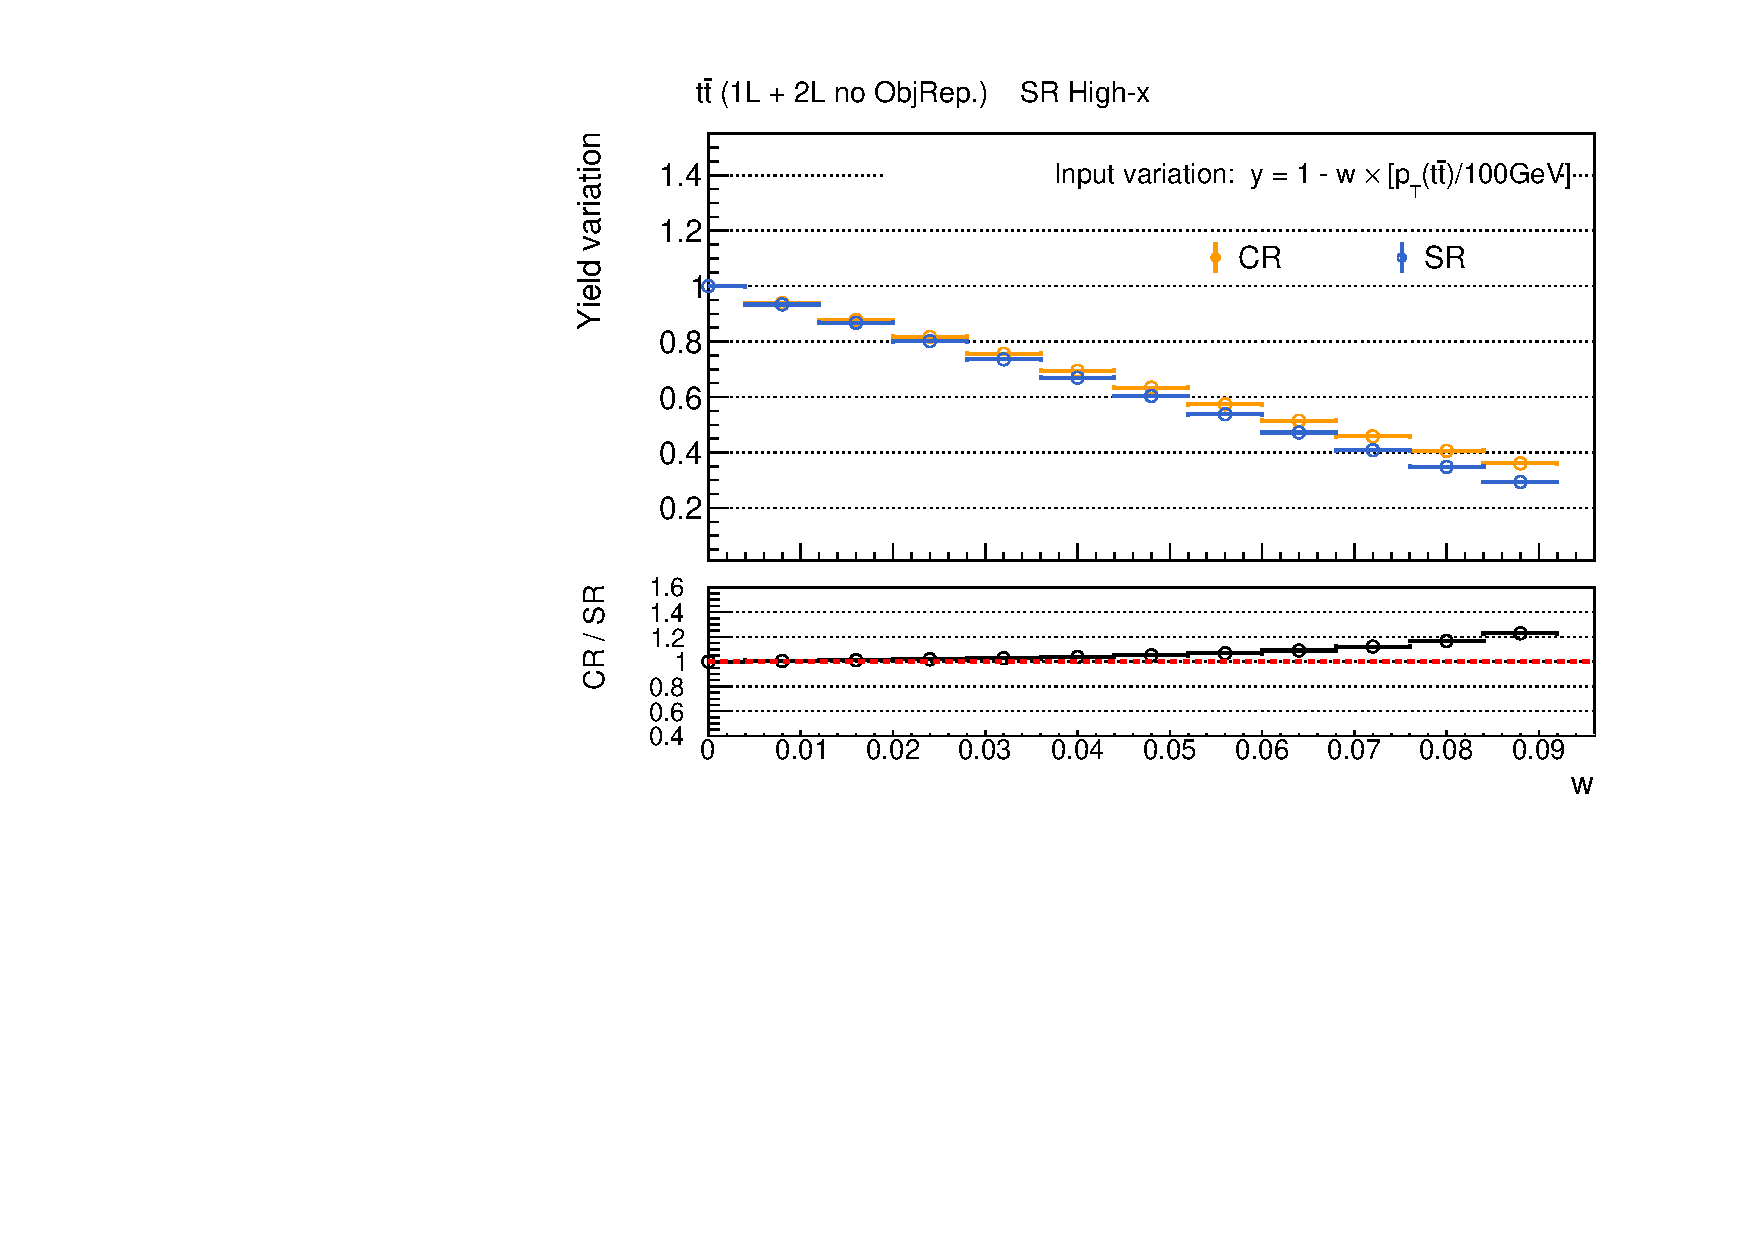
\includegraphics[width=0.488\textwidth]{figures/BGestimation/valid_extp/SFTF_ttNoObjRep_SRHighx_extp_varHighx__ttPt.pdf}}
 \caption{Extrapolation error in SR/CR (a)(b) Low-x, and (c)(d) High-x. B-tagging requirement is removed. Top pannels show the yield variation of $\wjets$ (left) and $\ttbar$ (right) when injecting the variation by reweighting the MC with Eq. \ref{eq::BGestimation::injected_MCvariation}. Bottom rows are the relative difference in their response against the injected variation, namely the extrapolation errir. For the $\ttbar$ process, component estimated by the object replacement method is removed.  \label{fig::BGestimation::valid_extp_6J} }
\end{figure}


%%%%%%%%%%%%%%%% 3B
\begin{figure}[h]
  \centering
    \subfigure[]{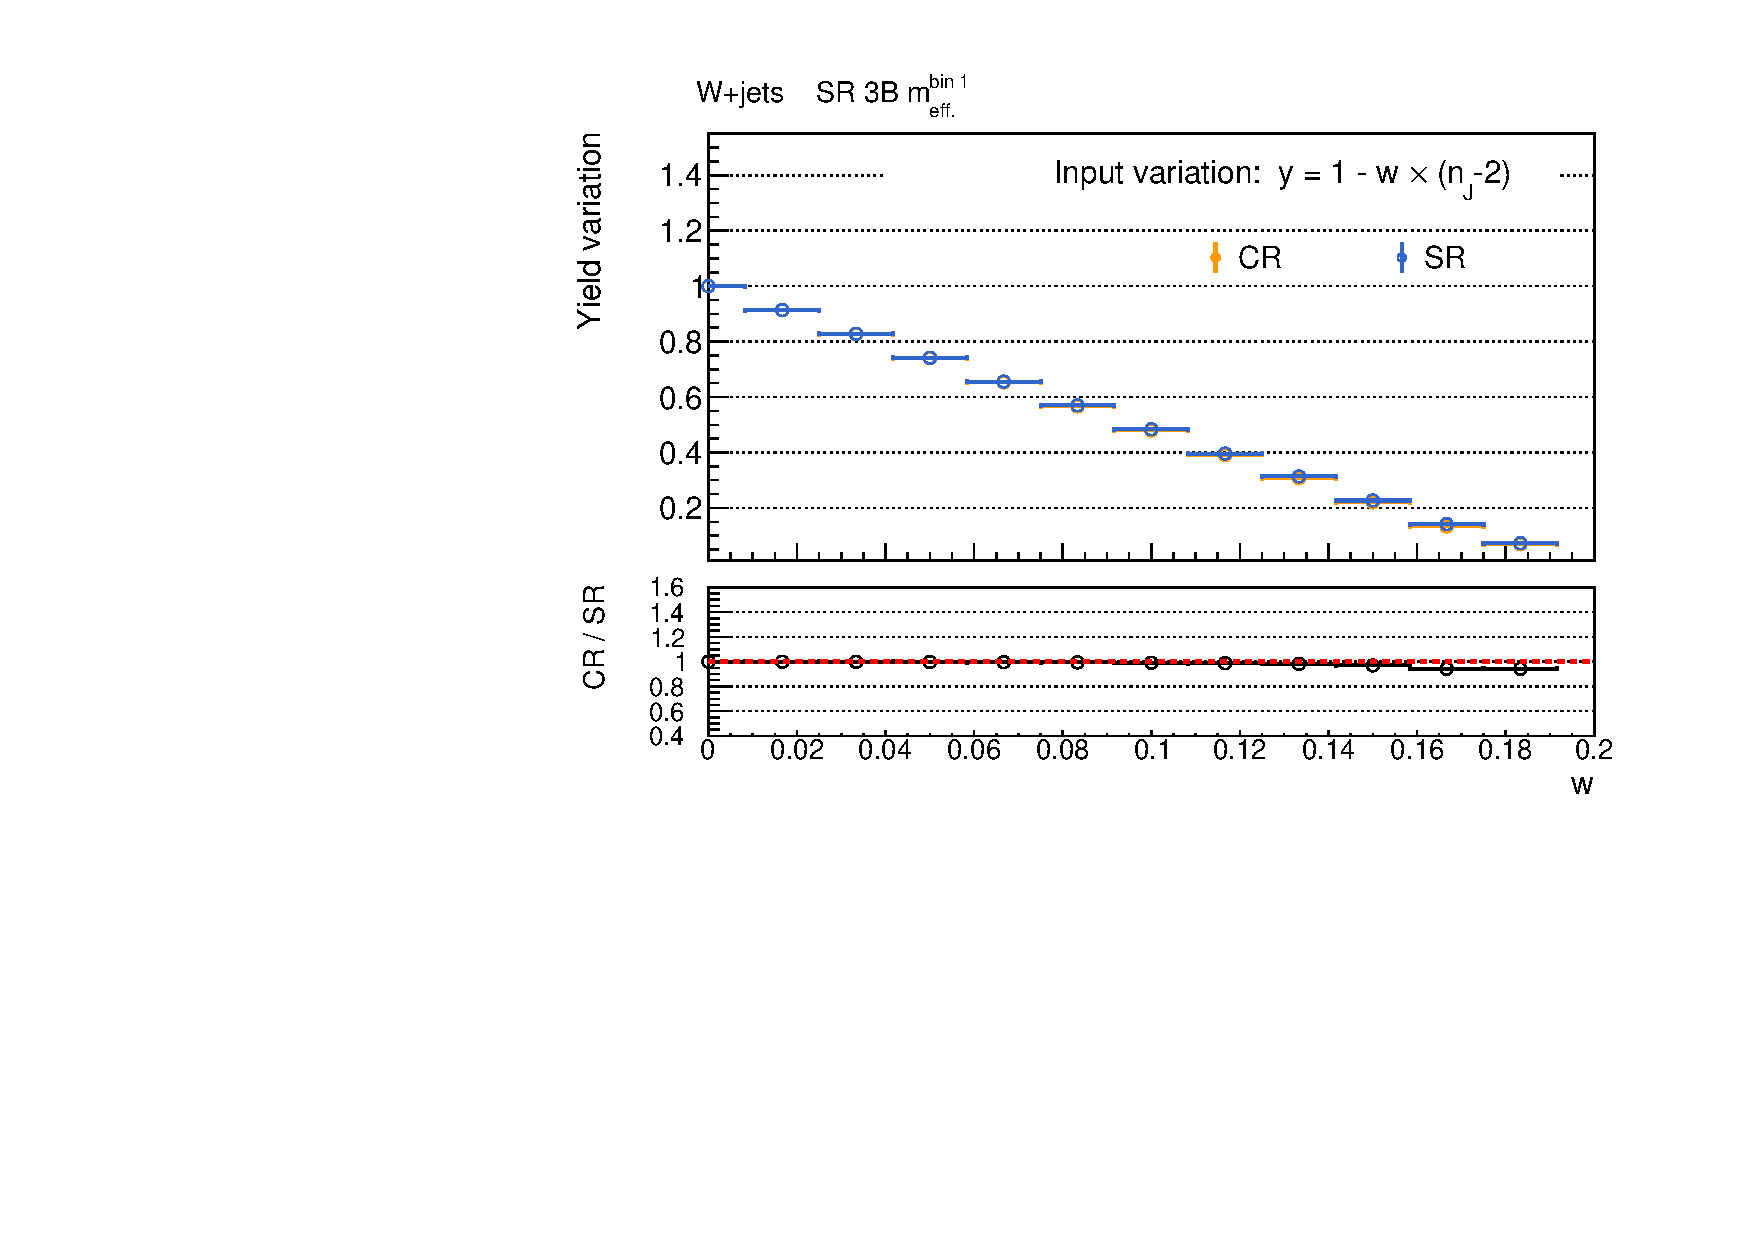
\includegraphics[width=0.488\textwidth]{figures/BGestimation/valid_extp/SFTF_wjets_SR3BMEFF1_extp_var3B__nJet30.pdf}}
    \subfigure[]{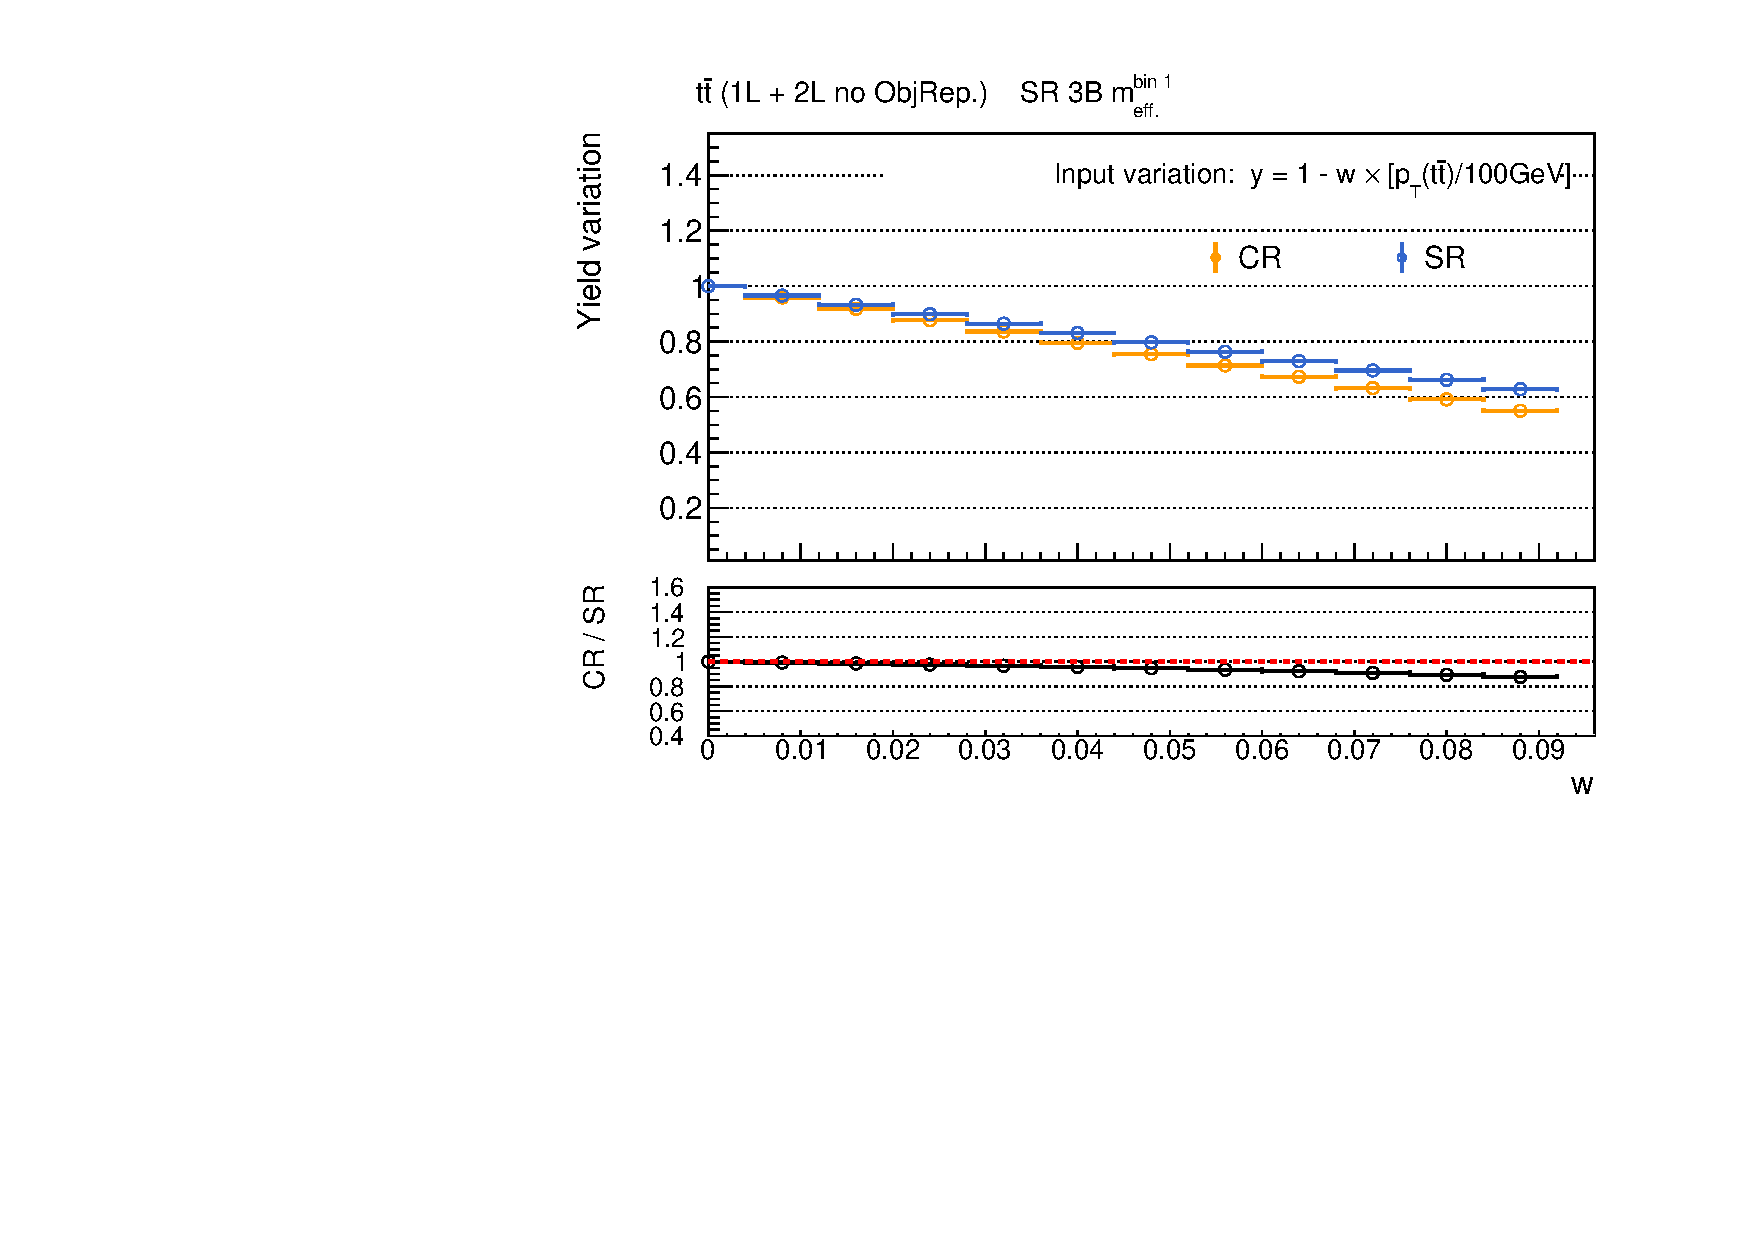
\includegraphics[width=0.488\textwidth]{figures/BGestimation/valid_extp/SFTF_ttNoObjRep_SR3BMEFF1_extp_var3B__ttPt.pdf}}
    \subfigure[]{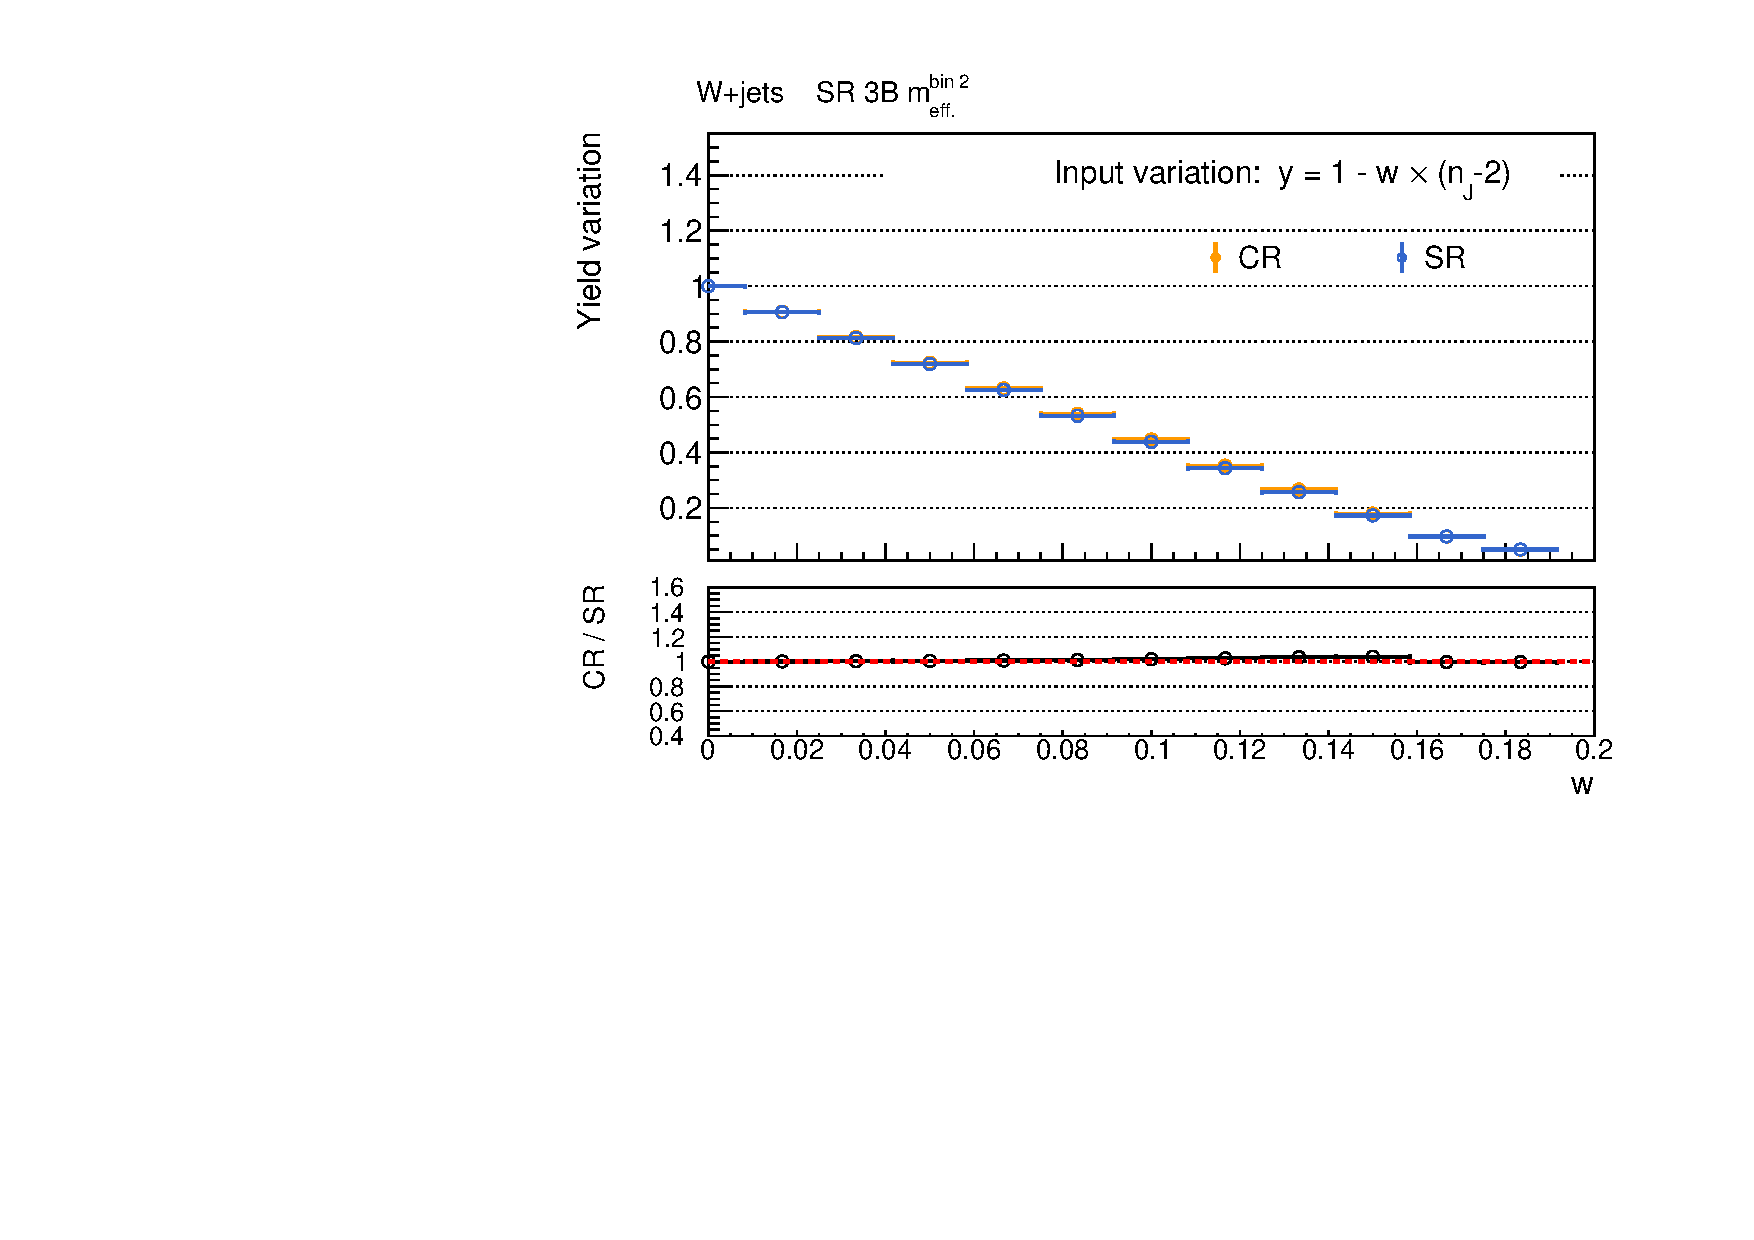
\includegraphics[width=0.488\textwidth]{figures/BGestimation/valid_extp/SFTF_wjets_SR3BMEFF2_extp_var3B__nJet30.pdf}}
    \subfigure[]{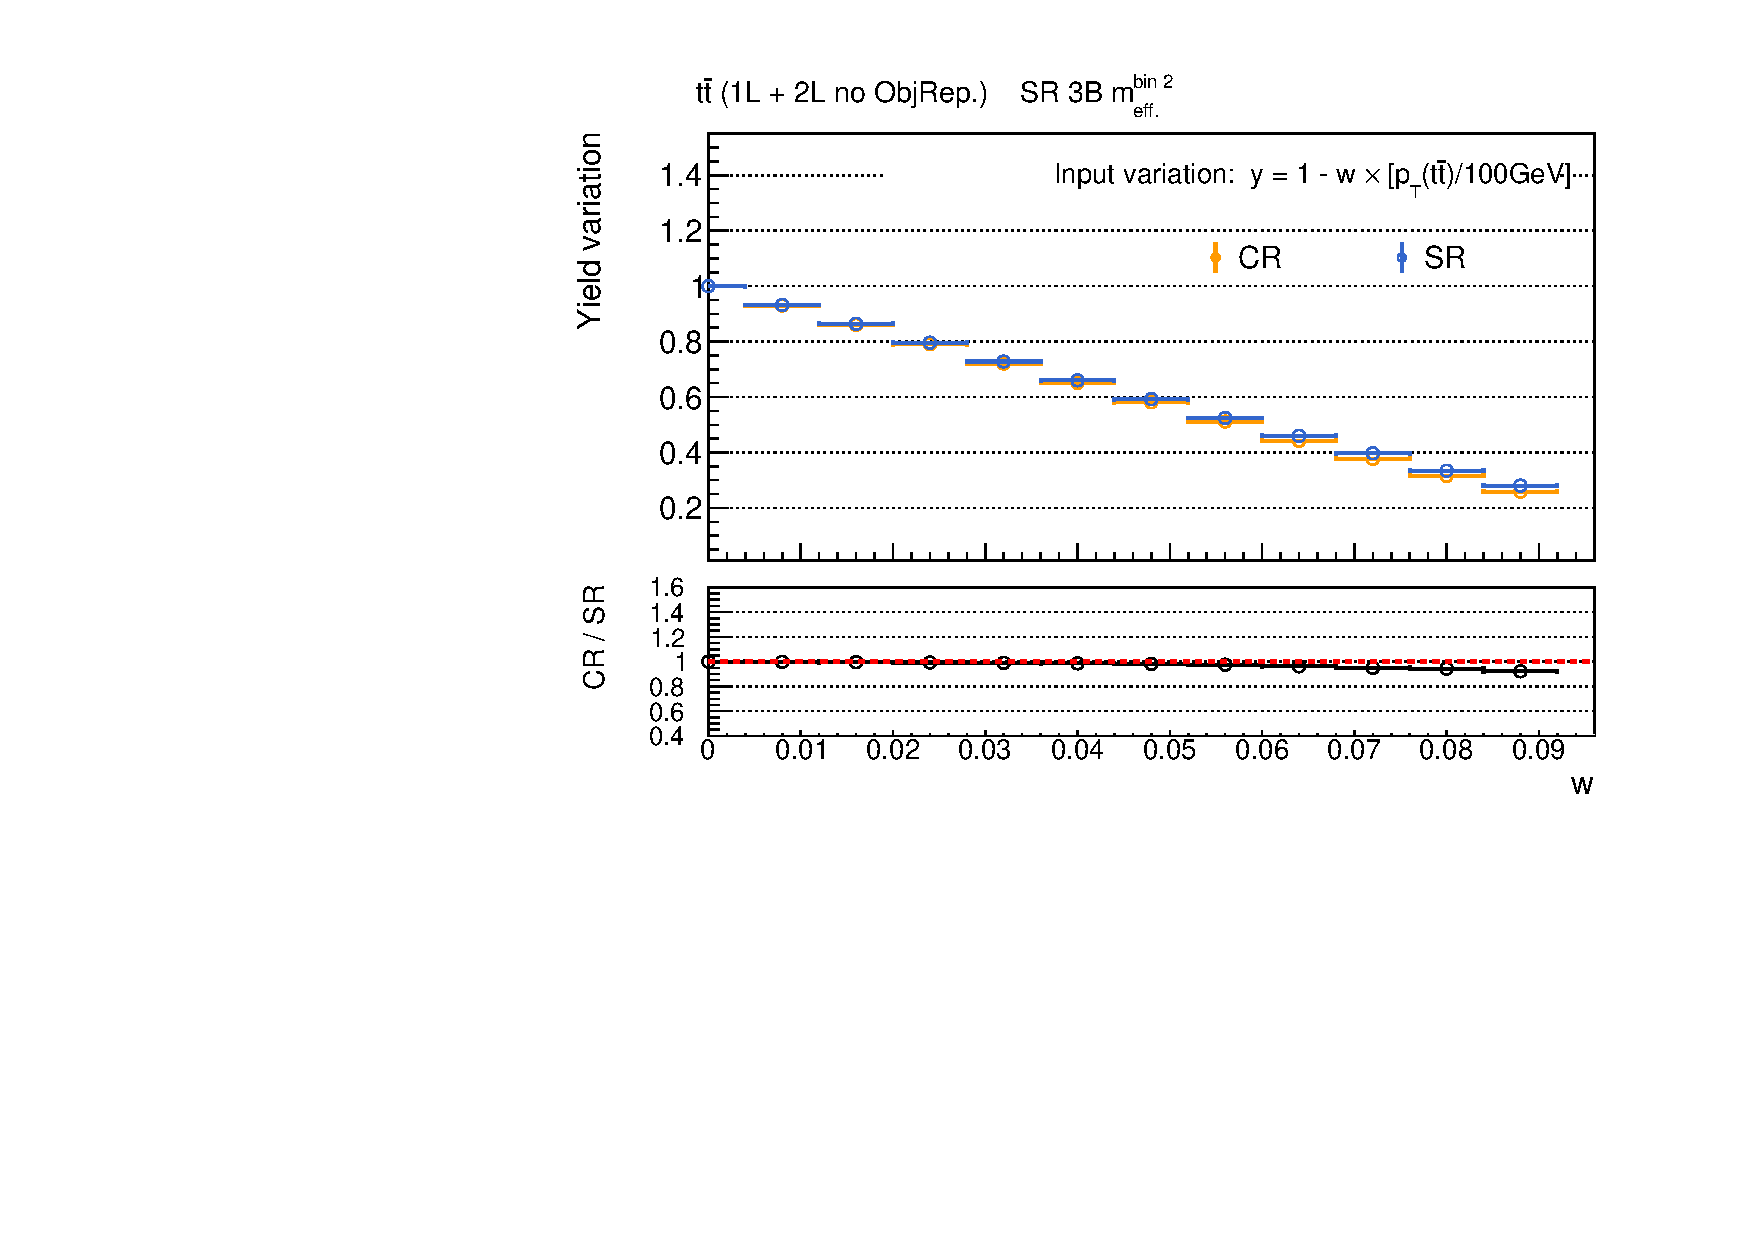
\includegraphics[width=0.488\textwidth]{figures/BGestimation/valid_extp/SFTF_ttNoObjRep_SR3BMEFF2_extp_var3B__ttPt.pdf}}
 \caption{Extrapolation error in SR/CR 3B. B-tagging requirement is removed for $\wjets$. Top pannels show the yield variation of $\wjets$ (left) and $\ttbar$ (right) when injecting the variation by reweighting the MC with Eq. \ref{eq::BGestimation::injected_MCvariation}. Bottom rows are the relative difference in their response against the injected variation, namely the extrapolation errir. For the $\ttbar$ process, component estimated by the object replacement method is removed.  \label{fig::BGestimation::valid_extp_3B} }
\end{figure}





%%%%%%%%%%%%%%%% VRa2J
\begin{figure}[h]
  \centering
    \subfig{0.488}{figures/BGestimation/valid_extp/SFTF_wjets_VRa2JMEFF1_extp_var2J__nJet30.pdf}{VRa/CR 2J $\meffIncFirst$ for $\wjets$}
    \subfig{0.488}{figures/BGestimation/valid_extp/SFTF_ttNoObjRep_VRa2JMEFF1_extp_var2J__ttPt.pdf}{VRa/CR 2J $\meffIncFirst$ for $\ttbar$}
    \subfig{0.488}{figures/BGestimation/valid_extp/SFTF_wjets_VRa2JMEFF2_extp_var2J__nJet30.pdf}{VRa/CR 2J $\meffIncSecond$ for $\wjets$}
    \subfig{0.488}{figures/BGestimation/valid_extp/SFTF_ttNoObjRep_VRa2JMEFF2_extp_var2J__ttPt.pdf}{VRa/CR 2J $\meffIncSecond$ for $\ttbar$}
    \subfig{0.488}{figures/BGestimation/valid_extp/SFTF_wjets_VRa2JMEFF3_extp_var2J__nJet30.pdf}{VRa/CR 2J $\meffIncThird$ for $\wjets$}
    \subfig{0.488}{figures/BGestimation/valid_extp/SFTF_ttNoObjRep_VRa2JMEFF3_extp_var2J__ttPt.pdf}{VRa/CR 2J $\meffIncThird$ for $\ttbar$}
 \caption{Extrapolation error in VRa/CR \textbf{2J} evaluated by reweighting the MC with Eq. (\ref{eq::BGestimation::injected_MCvariation}).  }
\label{fig::BGestimation::valid_extp_VRa2J} 
\end{figure}



%%%%%%%%%%%%%%%% VRa6J
\begin{figure}[h]
  \centering
    \subfig{0.488}{figures/BGestimation/valid_extp/SFTF_wjets_VRa6JMEFF1_extp_var6J__nJet30.pdf}{VRa/CR 6J $\meffIncFirst$ for $\wjets$}
    \subfig{0.488}{figures/BGestimation/valid_extp/SFTF_ttNoObjRep_VRa6JMEFF1_extp_var6J__ttPt.pdf}{VRa/CR 6J $\meffIncFirst$ for $\ttbar$}
    \subfig{0.488}{figures/BGestimation/valid_extp/SFTF_wjets_VRa6JMEFF2_extp_var6J__nJet30.pdf}{VRa/CR 6J $\meffIncSecond$ for $\wjets$}
    \subfig{0.488}{figures/BGestimation/valid_extp/SFTF_ttNoObjRep_VRa6JMEFF2_extp_var6J__ttPt.pdf}{VRa/CR 6J $\meffIncSecond$ for $\ttbar$}
    \subfig{0.488}{figures/BGestimation/valid_extp/SFTF_wjets_VRa6JMEFF3_extp_var6J__nJet30.pdf}{VRa/CR 6J $\meffIncThird$ for $\wjets$}
    \subfig{0.488}{figures/BGestimation/valid_extp/SFTF_ttNoObjRep_VRa6JMEFF3_extp_var6J__ttPt.pdf}{VRa/CR 6J $\meffIncThird$ for $\ttbar$}
 \caption{Extrapolation error in VRa/CR \textbf{6J} evaluated by reweighting the MC with Eq. (\ref{eq::BGestimation::injected_MCvariation}). }
  \label{fig::BGestimation::valid_extp_VRa6J} 
\end{figure}



%%%%%%%%%%%%%%%% Lowx/Highx/3B
\begin{figure}[h]
  \centering
    \subfig{0.46}{figures/BGestimation/valid_extp/SFTF_wjets_VRaLowx_extp_varLowx__nJet30.pdf}{VRa/CR Low-x for $\wjets$}
    \subfig{0.46}{figures/BGestimation/valid_extp/SFTF_ttNoObjRep_VRaLowx_extp_varLowx__ttPt.pdf}{VRa/CR Low-x for $\ttbar$}
    \subfig{0.46}{figures/BGestimation/valid_extp/SFTF_wjets_VRaHighx_extp_varHighx__nJet30.pdf}{VRa/CR High-x for $\wjets$}
    \subfig{0.46}{figures/BGestimation/valid_extp/SFTF_ttNoObjRep_VRaHighx_extp_varHighx__ttPt.pdf}{VRa/CR High-x for $\ttbar$}
    \subfig{0.46}{figures/BGestimation/valid_extp/SFTF_wjets_VRa3BMEFF1_extp_var3B__nJet30.pdf}{VRa/CR 3B $\meffIncFirst$ for $\wjets$}
    \subfig{0.46}{figures/BGestimation/valid_extp/SFTF_ttNoObjRep_VRa3BMEFF1_extp_var3B__ttPt.pdf}{VRa/CR 3B $\meffIncFirst$ for $\ttbar$}
    \subfig{0.46}{figures/BGestimation/valid_extp/SFTF_wjets_VRa3BMEFF2_extp_var3B__nJet30.pdf}{VRa/CR 3B $\meffIncSecond$ for $\wjets$}
    \subfig{0.46}{figures/BGestimation/valid_extp/SFTF_ttNoObjRep_VRa3BMEFF2_extp_var3B__ttPt.pdf}{VRa/CR 3B $\meffIncSecond$ for $\ttbar$}
 \caption{Extrapolation error in VRa/CR (a)(b) \textbf{Low-x}, (c)(d) \textbf{High-x} and (e-h) \textbf{3B} evaluated by reweighting the MC with Eq. (\ref{eq::BGestimation::injected_MCvariation}). }
\label{fig::BGestimation::valid_extp_Varx3B} 
\end{figure}

%%%%%%%%%%%%%%%% VRb2J
\begin{figure}[h]
  \centering
    \subfig{0.488}{figures/BGestimation/valid_extp/SFTF_wjets_VRb2JMEFF1_extp_var2J__nJet30.pdf}{VRb/CR 2J $\meffIncFirst$ for $\wjets$}
    \subfig{0.488}{figures/BGestimation/valid_extp/SFTF_ttNoObjRep_VRb2JMEFF1_extp_var2J__ttPt.pdf}{VRb/CR 2J $\meffIncFirst$ for $\ttbar$}
    \subfig{0.488}{figures/BGestimation/valid_extp/SFTF_wjets_VRb2JMEFF2_extp_var2J__nJet30.pdf}{VRb/CR 2J $\meffIncSecond$ for $\wjets$}
    \subfig{0.488}{figures/BGestimation/valid_extp/SFTF_ttNoObjRep_VRb2JMEFF2_extp_var2J__ttPt.pdf}{VRb/CR 2J $\meffIncSecond$ for $\ttbar$}
    \subfig{0.488}{figures/BGestimation/valid_extp/SFTF_wjets_VRb2JMEFF3_extp_var2J__nJet30.pdf}{VRb/CR 2J $\meffIncThird$ for $\wjets$}
    \subfig{0.488}{figures/BGestimation/valid_extp/SFTF_ttNoObjRep_VRb2JMEFF3_extp_var2J__ttPt.pdf}{VRb/CR 2J $\meffIncThird$ for $\ttbar$}
 \caption{Extrapolation error in VRb/CR \textbf{2J} evaluated by reweighting the MC with Eq. (\ref{eq::BGestimation::injected_MCvariation}).  }
\label{fig::BGestimation::valid_extp_VRb2J}
\end{figure}




%%%%%%%%%%%%%%%% VRb6J
\begin{figure}[h]
  \centering
    \subfig{0.488}{figures/BGestimation/valid_extp/SFTF_wjets_VRb6JMEFF1_extp_var6J__nJet30.pdf}{VRb/CR 6J $\meffIncFirst$ for $\wjets$}
    \subfig{0.488}{figures/BGestimation/valid_extp/SFTF_ttNoObjRep_VRb6JMEFF1_extp_var6J__ttPt.pdf}{VRb/CR 6J $\meffIncFirst$ for $\ttbar$}
    \subfig{0.488}{figures/BGestimation/valid_extp/SFTF_wjets_VRb6JMEFF2_extp_var6J__nJet30.pdf}{VRb/CR 6J $\meffIncSecond$ for $\wjets$}
    \subfig{0.488}{figures/BGestimation/valid_extp/SFTF_ttNoObjRep_VRb6JMEFF2_extp_var6J__ttPt.pdf}{VRb/CR 6J $\meffIncSecond$ for $\ttbar$}
    \subfig{0.488}{figures/BGestimation/valid_extp/SFTF_wjets_VRb6JMEFF3_extp_var6J__nJet30.pdf}{VRb/CR 6J $\meffIncThird$ for $\wjets$}
    \subfig{0.488}{figures/BGestimation/valid_extp/SFTF_ttNoObjRep_VRb6JMEFF3_extp_var6J__ttPt.pdf}{VRb/CR 6J $\meffIncThird$ for $\ttbar$}
 \caption{Extrapolation error in VRb/CR \textbf{6J} evaluated by reweighting the MC with Eq. (\ref{eq::BGestimation::injected_MCvariation}).   }
 \label{fig::BGestimation::valid_extp_VRb6J} 
\end{figure}



%%%%%%%%%%%%%%%% Lowx/Highx/3B
\begin{figure}[h]
  \centering
    \subfig{0.46}{figures/BGestimation/valid_extp/SFTF_wjets_VRbLowx_extp_varLowx__nJet30.pdf}{VRb/CR Low-x for $\wjets$}
    \subfig{0.46}{figures/BGestimation/valid_extp/SFTF_ttNoObjRep_VRbLowx_extp_varLowx__ttPt.pdf}{VRb/CR Low-x for $\ttbar$}
    \subfig{0.46}{figures/BGestimation/valid_extp/SFTF_wjets_VRbHighx_extp_varHighx__nJet30.pdf}{VRb/CR High-x for $\wjets$}
    \subfig{0.46}{figures/BGestimation/valid_extp/SFTF_ttNoObjRep_VRbHighx_extp_varHighx__ttPt.pdf}{VRb/CR High-x for $\ttbar$}
    \subfig{0.46}{figures/BGestimation/valid_extp/SFTF_wjets_VRb3BMEFF1_extp_var3B__nJet30.pdf}{VRb/CR 3B $\meffIncFirst$ for $\wjets$}
    \subfig{0.46}{figures/BGestimation/valid_extp/SFTF_ttNoObjRep_VRb3BMEFF1_extp_var3B__ttPt.pdf}{VRb/CR 3B $\meffIncFirst$ for $\ttbar$}
    \subfig{0.46}{figures/BGestimation/valid_extp/SFTF_wjets_VRb3BMEFF2_extp_var3B__nJet30.pdf}{VRb/CR 3B $\meffIncSecond$ for $\wjets$}
    \subfig{0.46}{figures/BGestimation/valid_extp/SFTF_ttNoObjRep_VRb3BMEFF2_extp_var3B__ttPt.pdf}{VRb/CR 3B $\meffIncSecond$ for $\ttbar$}
 \caption{Extrapolation error in VRb/CR (a)(b) \textbf{Low-x}, (c)(d) \textbf{High-x} and (e-h) \textbf{3B} evaluated by reweighting the MC with Eq. (\ref{eq::BGestimation::injected_MCvariation}). }
\label{fig::BGestimation::valid_extp_Varx3B} 
\end{figure}






